\documentclass[12pt]{article}
\usepackage{natbib}
\usepackage{siunitx}
\usepackage{url}
\usepackage{amssymb}
\usepackage{rotating}
\usepackage[utf8x]{inputenc}
\usepackage{amsmath}
\usepackage{cancel}
\usepackage{graphicx}
\graphicspath{{images/}}
\usepackage{parskip}
\usepackage{fancyhdr}
\usepackage{vmargin}
\usepackage{float}  
\usepackage{gensymb}
\usepackage{graphicx}
\usepackage{comment}
\usepackage{caption}
\usepackage{subcaption}
\usepackage[spanish]{babel}
\usepackage[final]{pdfpages}
\usepackage{times} 
\usepackage[spanish]{babel}
\usepackage{chemfig}
\usepackage{lscape}
\usepackage{mhchem}
\usepackage{modiagram}
\usepackage[belowskip=-10pt,aboveskip=2pt]{caption}
\usepackage[framed,numbered,autolinebreaks,useliterate]{mcode}
\usepackage{multicol}
\usepackage{hyperref}
\hypersetup{
    colorlinks,
    citecolor=black,
    filecolor=black,
    linkcolor=black,
    urlcolor=black
}

\usepackage{enumerate} 
\providecommand{\abs}[1]{\lvert#1\rvert}
\setmarginsrb{2 cm}{2 cm}{2 cm}{2 cm}{0.5 cm}{0.5 cm}{0.25 cm}{0.25 cm}

\title{Aplicación del método de Newton Raphson para describir la cinemática de un mecanismo}% Title
\author{}								% Author
\date{\today}											% Date

\makeatletter
\let\thetitle\@title
\let\theauthor\@author
\let\thedate\@date
\makeatother


\pagestyle{fancy}
\fancyhf{}
\rhead{\theauthor}
\lhead{\thetitle}
\cfoot{\thepage}
\renewcommand{\baselinestretch}{1}
\begin{document}


\begin{titlepage}
	\centering
    \vspace*{0.5 cm}
    
\includegraphics[scale = 0.13]{UNAL.png}\\[2.0 cm]	% University Logo
    \textsc{\LARGE Universidad Nacional de Colombia}\\[0.3 cm]	% University Name
    \textsc{Facultad de ingeniería}\\[0.6 cm]	% University Name
    \textsc{Departamento de ingeniería mecánica y mecatrónica}\\[0.6 cm]	
     \textsc{Métodos numéricos}\\[0.6 cm]
      \textsc{Grupo 2}\\[0.6 cm]
	\textsc{\Large 2021-1}\\[1 cm]				% Semestre
	\rule{\linewidth}{0.2 mm} \\[0.4 cm]
	{ \huge \bfseries \thetitle}\\
	\rule{\linewidth}{0.2 mm} \\[0.8 cm]
	
		\begin{minipage}{0.4\textwidth}
		\begin{flushleft} \large
			\emph{Autores:}\\
			Andrés Holguín R.\\
			Julián A. Caipa P.\\
			Santiago Marín B.
			
			\medskip
			\medskip
			\medskip
			\end{flushleft}
			\end{minipage}~
			\begin{minipage}{0.4\textwidth}
            
			\begin{flushright} \large
			\emph{Docente:} \\
			Ing. Oswaldo\\
			 Rojas Camacho
		\end{flushright}
        \end{minipage}
        
\newpage

\tableofcontents
\end{titlepage}


\newpage

\section{Objetivos}
\begin{itemize}
    \item Resolver un problema aplicado a la ingeniería implementando los conceptos adquiridos en el curso de métodos numéricos. 
    \item Realizar el proceso de resolución de mecanismos mediante el uso recurrente de métodos numéricos como procedimiento de solución del problema con el fin de optimizar la precisión de la solución y de los recursos computacionales asociados al mismo.
    \item Implementar el método de Newton Raphson para lograr determinar los perfiles cinemáticos del mecanismo a partir de un movimiento ejercido por el eje de un motor.
\end{itemize}
        \vspace{-10pt}
\section{Introducción y planteamiento del problema}
        \vspace{-10pt}
    \begin{figure} [H]
        \centerline{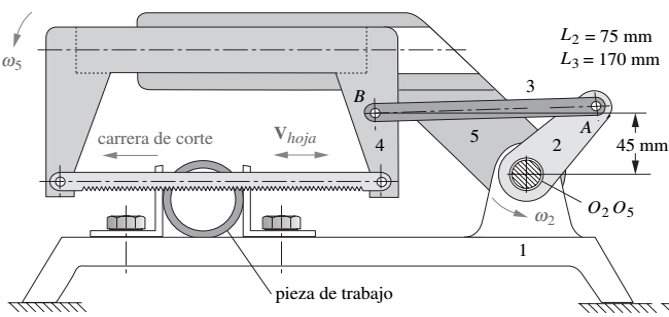
\includegraphics[width=10cm, height=10cm,keepaspectratio]{Sierra.png}}
        \caption{Mecanismo de trabajo tipo sierra eléctrica.}
        \vspace{-10pt}
        \label{Sierra}
    \end{figure}
Se tiene un mecanismo de tipo sierra eléctrica, utilizado para cortar barras de metal. Este trabaja mediante transmisión de movimiento radial a lineal a través de la conexión de sus diferentes eslabones.
Visto en la figura \ref{Sierra}, el movimiento radial empieza con el eje en el punto $1$, y termina en movimiento lineal en $4$, permitiendo el corte de la pieza. Se va a determinar el análisis cinemático completo del mecanismo a partir del análisis de su cadena cinemática, logrando describir la posición, velocidad y aceleración de sus componentes para cualquier condición \cite{mecanismo}. Esto es necesario para lograr realizar un análisis cinético, de resistencia y a fatiga, sin embargo, estos conceptos no se abarcan en este informe. De este modo, se describen los vectores y ángulos del sistema:
        \vspace{-10pt}
\begin{figure} [H]
        \centerline{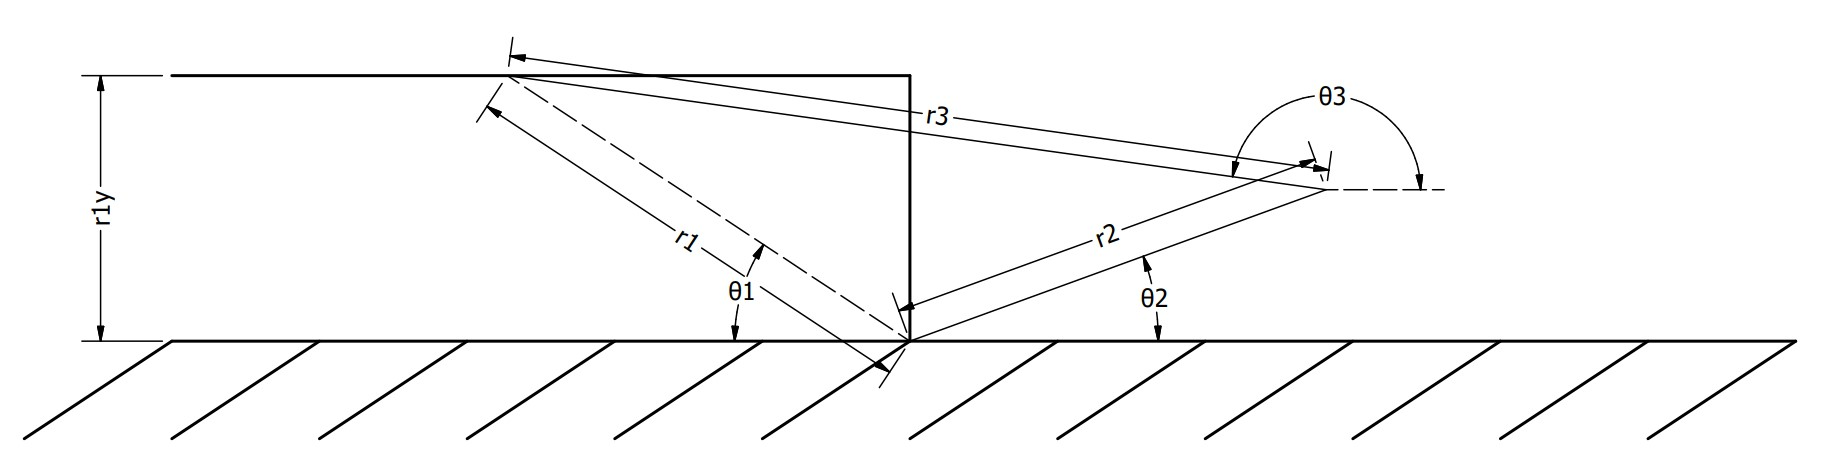
\includegraphics[width=14cm, height=12cm,keepaspectratio]{cadena cinematica.jpg}}
        \caption{Diagrama del sistema.}
        \label{cadena cinematica}
    \end{figure}
            \vspace{-15pt}
Donde:
    \begin{multicols}{3}
    \begin{itemize}
        \item $\vec{r_1}$: Eslabón formado por $\vec{r_2}+\vec{r_3}$.
        \item $V_r$: Velocidad lineal de $\vec{r_1}$.
        \item $A_r$: Aceleración lineal de $\vec{r_1}$.
        \item $\theta_1$: Ángulo de $\vec{r_1}$ respecto a la horizontal.
        \item $\omega_1$: Velocidad angular de $\theta_1$.
        \item $\alpha_1$: Aceleración angular de $\theta_1$.
        \item $\theta_3$: Ángulo de $\vec{r_3}$ respecto a la horizontal.
        \item $\omega_3$: Velocidad angular de $\theta_3$.
        \item $\alpha_3$: Aceleración angular de $\theta_3$.
    \end{itemize}
    \end{multicols}
\section{Marco teórico}
\subsection{Método de Newton Raphson}
\subsubsection{Método de Newton Raphson en una variable real}
El método de Newton Raphson es un método numérico abierto algorítmico que permite el calculo de raíces, inicialmente planteado para una función real, pero extrapolado, para una función en el dominio de los complejos, o un sistema de ecuaciones lineales o no lineales. Este método tiene diversas aplicaciones en el campo de la computación y en general, en cualquier campo de aplicación matemática de problemas de solución de raíces, máximos y mínimos, optimización, ceros de funciones notables, entre otros \cite{chapra}.

Inicialmente el método tiene la definición más sencilla en una función real $f$ y una aproximación inicial a la raíz $x_0$, llamado valor semilla, y que está considerablemente cerca a la raíz que se espera encontrar, para posteriormente aproximar la función utilizando su recta tangente en dicho punto utilizando cálculo diferencial, encontrando el intercepto de dicha línea con el eje $x$. Dicho intercepto será una mejor aproximación de la raíz que el supuesto inicial, por lo cual es posible iterar este procedimiento hasta encontrar el valor que aproxime de mejor forma a la raíz con la tolerancia de error definida para la aproximación. Formalmente el método se puede definir de la siguiente forma \cite{chapra}:

Sea $f$ de dominio y rango real una función diferenciable en el intervalo $(a,b)$, y una aproximación a la raíz de dicha función $x_n$, se puede encontrar una mejor aproximación $x_{n+1}$ que se puede deducir desde la recta tangente a la curva dada como:
\begin{equation*}
    y=f'(x_n)(x-x_n)+f(x_n)
    \label{recta tangente en x_n}
\end{equation*}
Evaluando para $(x,\;y)=(x_{n+1},\;0)$:
\begin{equation*}
    0=f'(x_n)(x_{n+1}-x_n)+f(x_n)
    \label{recta tangente en x_n+1}
\end{equation*}
Despejando para $x_{n+1}$:
\begin{equation*}
    x_{n+1}=x_n-\frac{f(x_n)}{f'(x_n)}
    \label{newton raphson 1var}
\end{equation*}
A partir de esta expresión se realiza el proceso iterativo de determinar $x_{n+1}$, sin embargo, se tienen ciertas condiciones de convergencia a tener en cuenta:
\begin{itemize}
    \item El valor semilla $x_0$ debe estar relativamente cerca a la raíz.
    \item El valor semilla $x_0$ no puede ser estacionario, esto quiere decir que su derivada no puede ser cero, ya que al evaluar en el algoritmo, se genera una división por cero.
    \item La derivada debe ser continua en el intervalo donde se encuentra la raíz.
\end{itemize}
Tratándose de un método abierto, el error absoluto y relativo asociado al NR se define como:
\begin{align}
    \varepsilon_{abs}=|x_{n+1}-x_n|&&&\varepsilon_{rel}=\frac{|x_{n+1}-x_n|}{|x_{n+1}|}
\end{align}
\subsubsection{Extrapolación del método a varias variables}
En el caso de sistemas de ecuaciones, el método emplea el uso de derivadas parciales para hacer el mismo algoritmo iterativo de aproximación mediante tangentes. La aproximación se realiza variable a variable de forma simultanea, por lo cual es necesario todas las derivadas parciales del sistema de ecuaciones \cite{mathews}. 

Dicho esto, se tiene un sistema de ecuaciones lineal o no lineal compatible determinado, descrito por el vector columna de funciones $F(x)$, diferenciable en $F:\mathbb{R}^k \rightarrow \mathbb{R}^k$, donde $x$ es el vector que contiene las variables del sistema, $x_n$ es el vector columna con los valores actuales de la iteración de las variables, y $x_{n+1}$ el vector columna que contiene los valores de la siguiente iteración. Para las derivadas, se aplica el concepto del Jacobiano del sistema, matriz que aplica un operador diferencial que permite derivar cada función respecto a cada variable y se obtienen los resultados en dicha matriz definida como:
\begin{equation*}
\scriptsize
    J_F(x)=\begin{pmatrix}
    \frac{\partial f_1(x)}{\partial x_1}&\frac{\partial f_1(x)}{\partial x_2}&...&\frac{\partial f_1(x)}{\partial x_k}\\ 
    \frac{\partial f_2(x)}{\partial x_1}&\frac{\partial f_2(x)}{\partial x_2}&...&\frac{\partial f_2(x)}{\partial x_k}\\ 
\vdots&\vdots&\ddots&\vdots\\
\frac{\partial f_k(x)}{\partial x_1}&\frac{\partial f_k(x)}{\partial x_2}&...&\frac{\partial f_k(x)}{\partial x_k}\\
    \end{pmatrix}
\end{equation*}
Ahora bien, aplicado al método, es necesario dividir por las derivadas en el algoritmo iterativo, por lo que se implementa la matriz inversa del Jacobiano, es decir, $J_F(x)^{-1}$. Finalmente, la ecuación iterativa para el método de Newton Raphson se da como:
\begin{equation}
    x_{n+1}=x_n-J_F(x_n)^{-1}\ F(x_n)
    \label{NR varias variables}
\end{equation}
Para el caso de varias variables, se puede determinar el error absoluto y relativo asociado a cada variable del vector $x_n$ y determinar la norma del vector compuesto por los errores determinados.
\section{Perfil cinemático del motor}
Como condiciones iniciales del sistema, se va a generar el perfil cinemático del eje del motor. Dicho esto, se establece que el eje va a partir del reposo y, durante el periodo de tiempo en que el eje del motor complete su primera revolución, va a tener una aceleración máxima de $5\;rad\;s^{-2}$. Para minimizar el jerk del motor, este periodo de tiempo va a separarse en tres periodos de misma longitud:
\begin{enumerate}
    \item Parte de aceleración en $0$, en aumento lineal hasta $5\;rad\;s^{-2}$.
    \item Se mantiene en $5\;rad\;s^{-2}$.
    \item Disminuye de $5\;rad\;s^{-2}$ hasta $0$.
\end{enumerate}
Después de haber ejercido la primera revolución, se va a mantener una velocidad angular constante $\omega_2 \approx6.45\;rad\;s^{-1}\;\approx 62\;rpm$, la cual es la resultante de esta aceleración. De este modo, se puede definir las ecuaciones de aceleración angular, y mediante procesos de integración, su velocidad y posición angular. A continuación se muestran los resultados:
\scriptsize
\begin{align}
\alpha_2(t)=&\left\lbrace \begin{array}{cl}
\frac{15\,t}{T} & \;\textrm{si}\;\;0\leq\;t<T/3\\
5 & \;\textrm{si}\;\;T/3\leq\;t\;\<2T/3\\
15-\frac{15\,t}{T} & \;\textrm{si}\;\;2T/3\leq\;t\;<T\\
0 & \;\textrm{si}\;\;T\le t
\end{array}\right. \label{MotorAce}\\
\omega_2(t)=&\left\lbrace \begin{array}{cl}
\frac{15\,t^2 }{2\,T}  & \;\textrm{si}\;\;0\leq\;t<T/3\\
5\,t-\frac{5\,T}{6} & \;\textrm{si}\;\;T/3\leq\;t\;<2T/3\\
15\,t-\frac{25\,T}{6}-\frac{15\,t^2 }{2\,T}  & \;\textrm{si}\;\;2T/3\leq\;t\;\leqT\\
\frac{10\,T}{3} & \;\textrm{si}\;\;T\le t
\end{array}\right.\label{MotorVel}\\
\theta_2(t)=&\left\lbrace \begin{array}{cl}
\frac{5\,t^3 }{2\,T}  & \;\textrm{si}\;\;0\leq\;t<T/3\\
\frac{5\,T^2 }{54}-\frac{5\,t\,{\left(T-3\,t\right)}}{6} & \;\textrm{si}\;\;T/3\leq\;t\;< 2T/3\\
\frac{5\,T^2 }{6}-\frac{25\,T\,t}{6}+\frac{15\,t^2 }{2}-\frac{5\,t^3 }{2\,T}  & \;\textrm{si}\;\;2T/3\leq\;t\;<T\\
\frac{10\,T\,t}{3}-\frac{5\,T^2 }{3} & \;\textrm{si}\;\;T\le t
\end{array}\right.\label{motorPos}
\end{align}
\normalsize
Con base a los resultados obtenidos en \eqref{motorPos}, es posible determinar el tiempo $T$ en que el eje realiza la primera revolución. Dado que $\theta_2(T)=2\pi$, se soluciona para esta condición, determinando que $T=1.942\;s$. A partir de este resultado se grafican los valores de tiempo el perfil cinemático del eje del motor para un tiempo $2T$, con el fin de evidenciar el motor a velocidad constante.
    \begin{figure} [H]
        \centerline{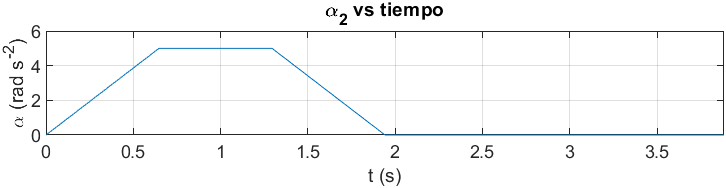
\includegraphics[width=9cm, height=12cm,keepaspectratio]{Perfiles/perfil cinematico aceleracion.png}}
        \label{}
    \end{figure}
    \vspace{-25pt}
        \begin{figure} [H]
        \centerline{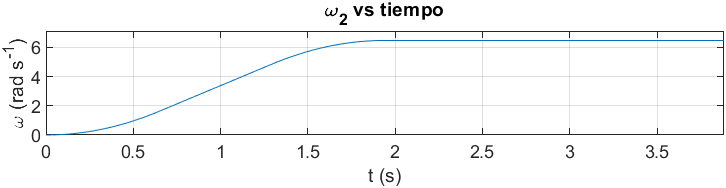
\includegraphics[width=9cm, height=12cm,keepaspectratio]{Perfiles/perfil cinematico velocidad.png}}
        \label{}
    \end{figure}
        \vspace{-25pt}
        \begin{figure} [H]
        \centerline{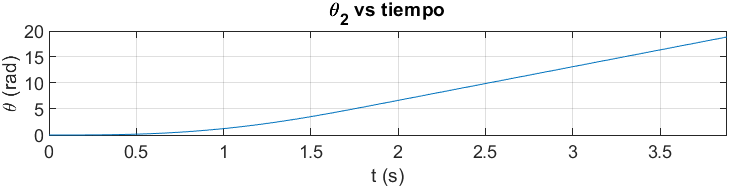
\includegraphics[width=9cm, height=12cm,keepaspectratio]{Perfiles/perfil cinematico posicion.png}}
        \caption{Perfil cinemático del eje del motor.}
        \label{}
    \end{figure}
\section{Resolución del problema}
\subsection{Cadena cinemática} \label{secCadenaCinematica}
Para poder solucionar el problema, lo primero es definir la cadena cinemática definida por los vectores del problema a partir de la figura \ref{cadena cinematica}. A continuación se evidencia la expresión correspondiente:
\begin{equation}
    \vec{r_1}=\vec{r_2}+\vec{r_3} \label{eqCad}
\end{equation}
A partir de \eqref{eqCad} se pueden definir las ecuaciones de posición respecto a las variables deseadas del sistema. Sumado a esto, igualando las ecuaciones a 0 y mediante procesos de derivación de las mismas, se pueden determinar los perfiles cinemáticos de las variables.
\subsubsection{Posición}
Con las condiciones dadas del problema, se pueden definir dos ecuaciones dimensionales respecto a los ejes coordenados $x$ y $y$ e igualarlas a 0. Adicionalmente, se debe plantear la ecuación de ligadura entre $r_1$ y $\theta_1$. Teniendo en cuenta que $r_1$, $\theta_1$ $\theta_2$ y $\theta_3$ varían en el tiempo, se tiene que:
\footnotesize
\begin{align}
        Fx(t)=0=&-r_1(t)Cos(\theta_1(t))+r_2Cos(\theta_2(t))+r_3Cos(\theta_2(t))
    \label{pos x}\\
        Fy(t)=0=&r_1Sen(\theta_1(t))-r_2Sen(\theta_2(t))-r_3Sen(\theta_2(t))
    \label{pos y}\\
        Fc(t)=0=&r_1(t)Sen(\theta_1(t))-r_{1y}
    \label{pos lig}
\end{align}
\normalsize
\subsubsection{Velocidad}
Para las ecuaciones de velocidad basta con derivar las ecuaciones de posición respecto al tiempo.
\footnotesize
\begin{align}
        \frac{\partial Fx(t)}{\partial t}=0=&\omega_1 \,r_1 \,\mathrm{sin}\left(\theta_1 \right)-V_r \,\mathrm{cos}\left(\theta_1 \right)-\omega_2 \,r_2 \,\mathrm{sin}\left(\theta_2 \right)-\omega_3 \,r_3 \,\mathrm{sin}\left(\theta_3 \right)
    \label{vel x}\\
        \frac{\partial Fy(t)}{\partial t}=0=&V_r \,\mathrm{sin}\left(\theta_1 \right)+\omega_1 \,r_1 \,\mathrm{cos}\left(\theta_1 \right)-\omega_2 \,r_2 \,\mathrm{cos}\left(\theta_2 \right)-\omega_3 \,r_3 \,\mathrm{cos}\left(\theta_3 \right)
    \label{vel y}\\
        \frac{\partial Fc(t)}{\partial t}=0=&V_r \,\mathrm{sin}\left(\theta_1 \right)+\omega_1 \,r_1 \,\mathrm{cos}\left(\theta_1 \right)
    \label{vel lig}
\end{align}
\normalsize
\subsubsection{Aceleración}
Para determinar la aceleración, se derivan las funciones de velocidad.
\begin{equation}
\footnotesize
    \begin{split}
    \frac{\partial^2 Fx(t)}{\partial t^2}=0=r_1 \,\mathrm{cos}\left(\theta_1 \right)\,{\omega_1 }^2 +2\,V_r \,\mathrm{sin}\left(\theta_1 \right)\,\omega_1 -r_2 \,\mathrm{cos}\left(\theta_2 \right)\,{\omega_2 }^2 -r_3 \,\mathrm{cos}\left(\theta_3 \right)\,{\omega_3 }^2\\
        -a_r \,\mathrm{cos}\left(\theta_1 \right)+\alpha_1 \,r_1 \,\mathrm{sin}\left(\theta_1 \right)-\alpha_2 \,r_2 \,\mathrm{sin}\left(\theta_2 \right)-\alpha_3 \,r_3 \,\mathrm{sin}\left(\theta_3 \right)
    \end{split}    \label{ac x}
\end{equation}
\begin{equation}
\footnotesize
    \begin{split}
       \frac{\partial^2 Fy(t)}{\partial t^2}=0=-r_1 \,\mathrm{sin}\left(\theta_1 \right)\,{\omega_1 }^2 +2\,V_r \,\mathrm{cos}\left(\theta_1 \right)\,\omega_1 +r_2 \,\mathrm{sin}\left(\theta_2 \right)\,{\omega_2 }^2 +r_3 \,\mathrm{sin}\left(\theta_3 \right)\,{\omega_3 }^2\\
       +a_r \,\mathrm{sin}\left(\theta_1 \right)+\alpha_1 \,r_1 \,\mathrm{cos}\left(\theta_1 \right)-\alpha_2 \,r_2 \,\mathrm{cos}\left(\theta_2 \right)-\alpha_3 \,r_3 \,\mathrm{cos}\left(\theta_3 \right)
    \end{split}\label{ac y}
\end{equation}
\begin{equation}
\footnotesize
    \frac{\partial^2 Fc(t)}{\partial t^2}=0=-r_1\, \mathrm{sin}\left(\theta_1\right) \omega_1^2\, + \,2 \, V_r \, \mathrm{cos}\left(\theta_1\right)\, \omega_1\, +\,  a_r\, \mathrm{sin}\left(\theta_1\right)\,  +\, \alpha_1 \,  r_1\, \mathrm{cos}\left(\theta_1\right)
    \label{ac lig}
\end{equation}
\subsection{Implementación del método de Newton Raphson}
Con las ecuaciones del sistema definidas, se puede implementar el método de Newton Raphson para resolver las variables deseadas, con una cota de error $\varepsilon<10^{-6}$. Inicialmente se trabajará el método de forma consecutiva, es decir, se resolverán las variables de posición, y se utilizarán sus valores como entradas para la resolución de la velocidad, y de la misma forma con los resultados de velocidad para la aceleración. Luego se realizará una segunda forma de aplicar el método, resolviendo las nueve variables de forma simultanea.

A partir de unas condiciones iniciales del motor en reposo: $\theta_2=0$, $\omega_2=0$ y $\alpha_2=0$, con valores de las constantes del sistema $r_{1y}$, $r_2$ y $r_3$ de $45\;mm,\;75\;mm$ y $170\;mm$ respectivamente, se va a tomar un valor semilla:
\footnotesize
\begin{equation}
    x_0=\begin{pmatrix}
r_1\\ 
\theta_1\\ 
\theta_3\\ 
v_r\\ 
\omega_1\\ 
\omega_3\\ 
a_r\\ 
\alpha_1\\ 
\alpha_3
\end{pmatrix}=\begin{pmatrix}
-0.1\\ 
-0.5\\ 
3\\ 
0.5\\ 
0\\ 
-0.5\\ 
0.5\\ 
0\\ 
-0.5
\end{pmatrix} \begin{bmatrix}
m\\ 
rad\\ 
rad\\ 
m\ s^{-1}\\ 
rad\ s^{-1}\\ 
rad\ s^{-1}\\ 
m\ s^{-2}\\ 
rad\ s^{-2}\\ 
rad\ s^{-2}
\end{bmatrix}
\end{equation}
\normalsize
Se toman estos valores medianamente alejados de la solución para que se evidencie la convergencia mediante el método.
\subsubsection{NR Consecutivo}\label{SecNRC}
Aplicando el método de Newton Raphson definido por \eqref{NR varias variables}, se implementan las expresiones de \eqref{pos x}, \eqref{pos y} y \eqref{pos lig} como el vector $F(x_n)$. Definiendo el jacobiano para $F(x_n)$ como:
\footnotesize
\begin{equation}
    J_{pos}=\left(\begin{array}{ccc}
\mathrm{sin}\left(\theta_1 \right) & r_1 \,\mathrm{cos}\left(\theta_1 \right) & 0\\
0 & r_{\textrm{1y}} \,{\left({\mathrm{cot}\left(\theta_1 \right)}^2 +1\right)} & -r_3 \,\mathrm{sin}\left(\theta_3 \right)\\
0 & 0 & -r_3 \,\mathrm{cos}\left(\theta_3 \right)
\end{array}\right)
\label{jacobiano pos}
\end{equation}
\normalsize
Y su Jacobiano inverso que se encuentra en el Anexo C.1.

Con todo y lo anterior, se realiza el proceso iterativo para la solución del sistema, obteniendo las siguientes gráficas de la convergencia de las variables de posición $r_1$, $\theta_1$ y $\theta_3$, con sus respectivos errores por variable, y el error total:
\begin{figure}[H]
\centering
  \begin{subfigure}[b]{0.49\textwidth}
    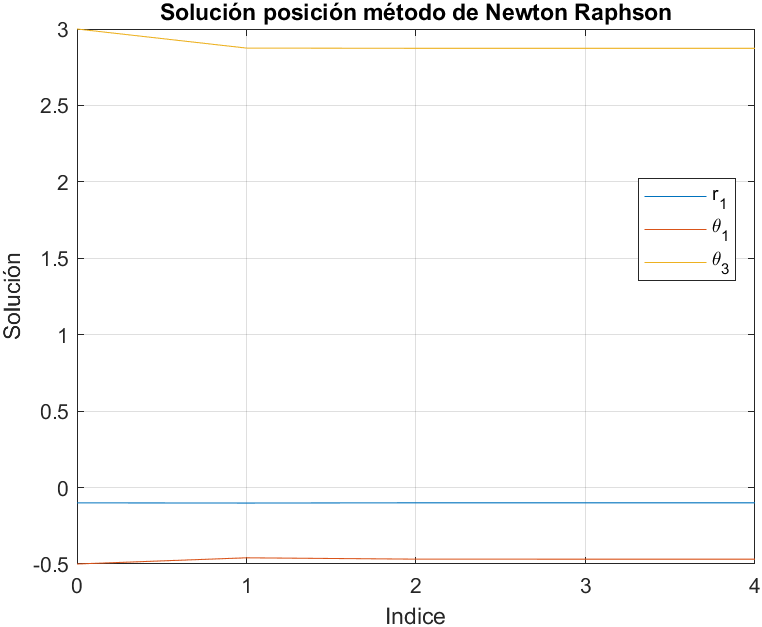
\includegraphics[width=7.5 cm, height=7.5 cm, keepaspectratio]{Implementacion/solucion pos NR.png}
    \caption{Convergencia de las variables de posición.}
    \label{}
  \end{subfigure}
  \hfill
  \begin{subfigure}[b]{0.49\textwidth}
    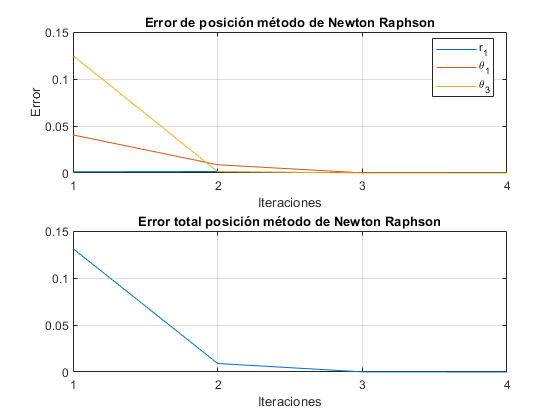
\includegraphics[width=8.5 cm, height=8.5 cm, keepaspectratio]{Implementacion/error pos NR.png}
    \caption{Errores de las variables de posición.}
    \label{}
  \end{subfigure}\\
  \vspace{10pt}
  \caption{Resultados del método de NR para la posición.}
\end{figure}
Después de 4 iteraciones, se tiene que:
\begin{align*}
r_1=-0.099672\;m&&\theta_1=-0.468422\;rad&&\theta_3=2.873694\;rad
\end{align*}
Para resolver las velocidades, se utilizan las ecuaciones \eqref{vel x},\eqref{vel y} y \eqref{vel lig} para formar $F(x_n)$, y se define su matriz Jacobiana (su Jacobiano inverso se encuentra en el Anexo C.2):
\footnotesize
\begin{equation}
    J_{vel}=\left(\begin{array}{ccc}
-\mathrm{cos}\left(\theta_1 \right) & r_1 \,\mathrm{sin}\left(\theta_1 \right) & -r_3 \,\mathrm{sin}\left(\theta_3 \right)\\
\mathrm{sin}\left(\theta_1 \right) & r_1 \,\mathrm{cos}\left(\theta_1 \right) & -r_3 \,\mathrm{cos}\left(\theta_3 \right)\\
\mathrm{sin}\left(\theta_1 \right) & r_1 \,\mathrm{cos}\left(\theta_1 \right) & 0
\end{array}\right)
\label{jacobiano vel}
\end{equation}
\normalsize
Al implementar el método descrito en \eqref{NR varias variables} y los valores semilla dados, se obtienen los resultados para $V_r$, $\omega_1$ y $\omega_3$:
\begin{figure}[H]
\centering
  \begin{subfigure}[b]{0.49\textwidth}
    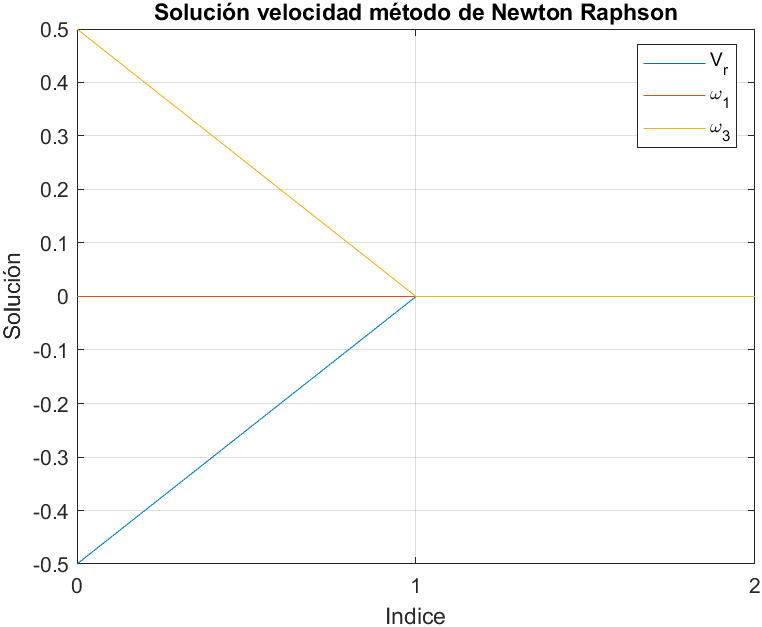
\includegraphics[width=7.5 cm, height=7.5 cm, keepaspectratio]{Implementacion/solucion vel NR.png}
    \caption{Convergencia de las variables de velocidad.}
    \label{}
  \end{subfigure}
  \hfill
  \begin{subfigure}[b]{0.49\textwidth}
    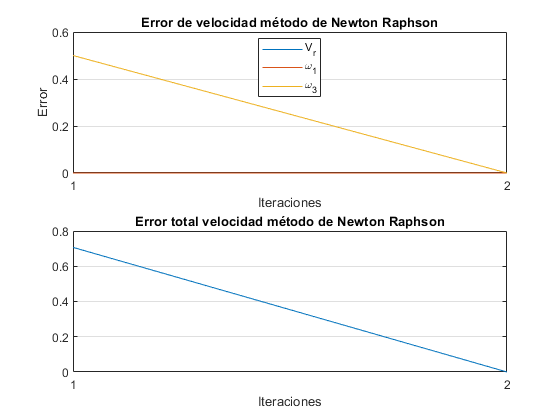
\includegraphics[width=8.5 cm, height=8.5 cm, keepaspectratio]{Implementacion/error vel NR.png}
    \caption{Errores de las variables de velocidad.}
    \label{}
  \end{subfigure}\\
  \vspace{10pt}
  \caption{Resultados del método de NR para la velocidad.}
\end{figure}
Después de 2 iteraciones, se tiene que:
\begin{align*}
V_1=0\;m\;s^{-1}&&\omega_1=0\;rad\;s^{-1}&&\omega_3=0\;rad\;s^{-1}
\end{align*}
Finalmente, para los valores de aceleración, utilizando \eqref{ac x}, \eqref{ac y} y \eqref{ac lig} para formar $F(x_n)$, se define su Jacobiano (y su Jacobiano que se encuentra en el Anexo C.3) como:
\footnotesize
\begin{equation}
J_{ac}=\left(\begin{array}{ccc}
\mathrm{sin}\left(\theta_1 \right) & r_1 \,\mathrm{cos}\left(\theta_1 \right) & 0\\
-\mathrm{cos}\left(\theta_1 \right) & r_1 \,\mathrm{sin}\left(\theta_1 \right) & -r_3 \,\mathrm{sin}\left(\theta_3 \right)\\
\mathrm{sin}\left(\theta_1 \right) & r_1 \,\mathrm{cos}\left(\theta_1 \right) & -r_3 \,\mathrm{cos}\left(\theta_3 \right)
\end{array}\right)
    \label{jacobiano ac}
\end{equation}
\normalsize
Al aplicar el método de NR con los valores semilla, se obtienen los siguientes resultados para $A_r$, $\alpha_1$ y $\alpha_3$:
\vspace{-10pt}
\begin{figure}[H]
\centering
  \begin{subfigure}[b]{0.49\textwidth}
    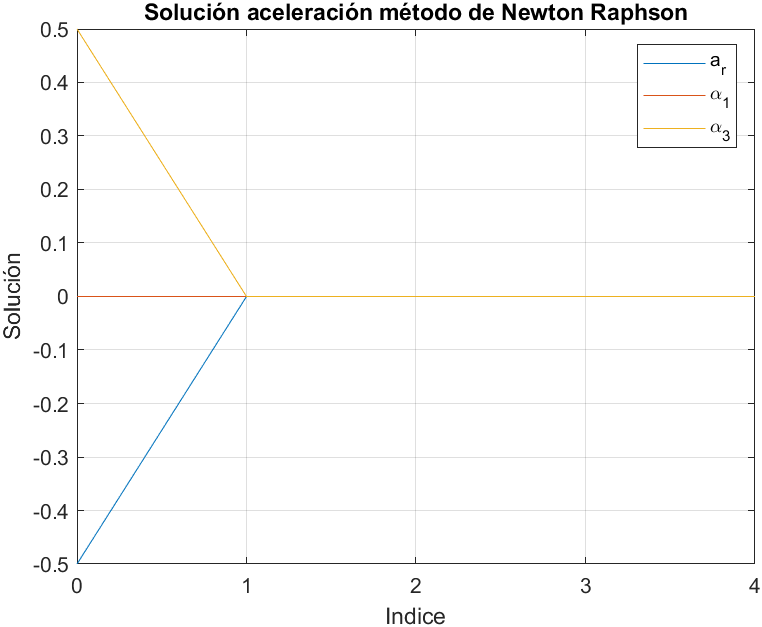
\includegraphics[width=7 cm, height=7 cm, keepaspectratio]{Implementacion/solucion ace NR.png}
    \caption{Convergencia de las variables de aceleración.}
    \label{}
  \end{subfigure}
  \hfill
  \begin{subfigure}[b]{0.49\textwidth}
    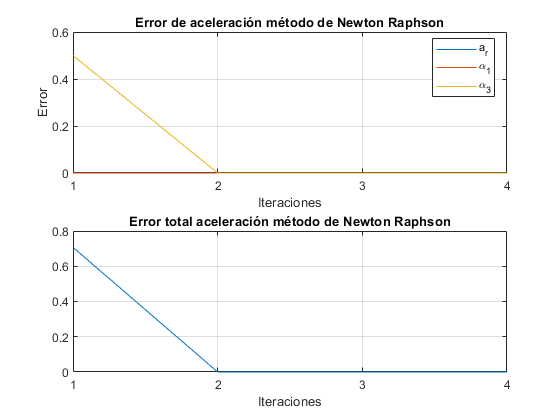
\includegraphics[width=7.5 cm, height=7.5 cm, keepaspectratio]{Implementacion/error ace NR.png}
    \caption{Errores de las variables de aceleración.}
    \label{}
  \end{subfigure}\\
      \vspace{10pt}
  \caption{Resultados del método de NR para la aceleración.}
\end{figure}
\vspace{-10pt}
Después de 4 iteraciones, se tiene que:
\vspace{-5pt}
\begin{align*}
A_r=0\;m\;s^{-2}&&\alpha_1=0\;rad\;s^{-2}&&\alpha_3=0\;rad\;s^{-2}
\end{align*}
\vspace{-35pt}
\subsubsection{NR Simultaneo}\label{SecNRS}
Ahora bien, estudiando el método de NR, fue posible determinar que el sistema se puede resolver llevando a cabo una implementación simultanea de las nueve ecuaciones que describen la cinemática general del sistema. A pesar de que las soluciones de velocidad y aceleración dependan de valores de posición, y de posición y velocidad respectivamente, a partir del valor semilla y de la convergencia de la posición, se converge simultáneamente a la solución de velocidad, y del mismo modo para la aceleración. Debido a que el sistema se resuelve en simultaneo, $F(x_n)$ se define con las nueve ecuaciones de cinemática, su Jacobiano de tamaño $9\times9$ se encuentra en el anexo \ref{JAC9}, debido a la extensión del inverso del Jacobiano, no se anexa al documento. Con todo y lo anterior, se obtienen los siguientes resultados:
\vspace{-10pt}
\begin{figure}[H]
\centering
  \begin{subfigure}[b]{0.49\textwidth}
    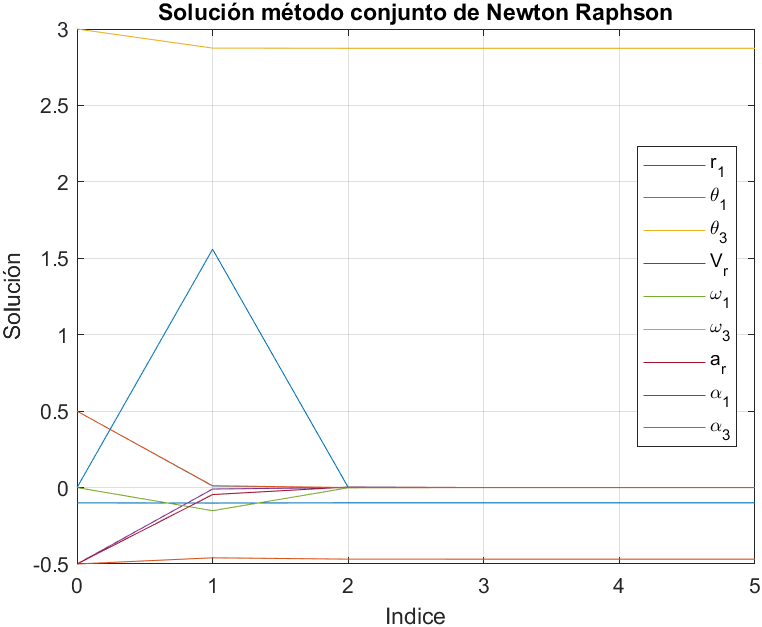
\includegraphics[width=7 cm, height=7 cm, keepaspectratio]{Implementacion/solucion NR conjunto.png}
    \caption{Convergencia de las variables en simultaneo.}
    \label{}
  \end{subfigure}
  \hfill
  \begin{subfigure}[b]{0.49\textwidth}
    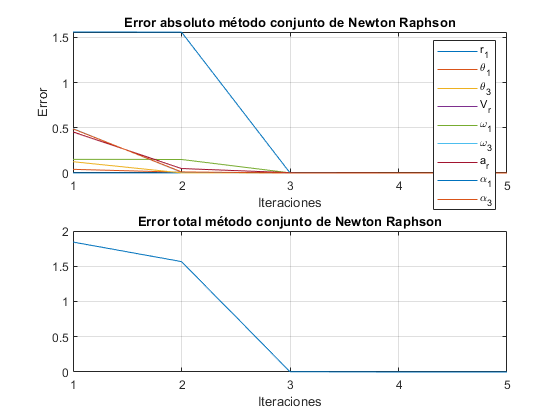
\includegraphics[width=7.5 cm, height=7.5 cm, keepaspectratio]{Implementacion/error NR conjunto.png}
    \caption{Errores de las variables en simultaneo.}
    \label{}
  \end{subfigure}\\
        \vspace{10pt}
  \caption{Resultados del método de NR en simultaneo.}
\end{figure}
Después de cinco iteraciones, se tiene que los valores finales son:
\begin{align*}
r_1=-0.099672\;m&&\theta_1=-0.468422\;rad&&\theta_3=2.873694\;rad\\
V_r=0\;m\;s^{-1}&&\omega_1=0\;rad\;s^{-1}&&\omega_3=0\;rad\;s^{-1}\\
A_r=0\;m\;s^{-2}&&\alpha_1=0\;rad\;s^{-2}&&\alpha_3=0\;rad\;s^{-2}
\end{align*}
Comparando estos resultados con los encontrados de manera consecutiva, se evidencia que ambos métodos convergen a la misma solución.
\subsection{Solución analítica}\label{solAna}
A pesar de que el problema se va a solucionar implementando el método de Newton Raphson, es importante tener la solución analítica al problema.
Esto se va a realizar porque es necesario comparar los resultados obtenidos por el método de NR con los valores exactos del sistema, para determinar el error real obtenido en la solución. Además, si se fueran a comparar los resultados del NR directamente con los resultados de simulación se pueden tener errores de medición, debido a las limitaciones de los software como \textit{Inventor}.

Dicho esto, a partir de las ecuaciones encontradas en la sección \ref{secCadenaCinematica}, es posible determinar las soluciones analíticas para las nueve variables del sistema. Estas ecuaciones se determinan mediante procedimientos matemáticos que no se van a profundizar en el informe. 
\footnotesize
\begin{align}
    \theta_3=&\pi -\mathrm{asin}\left(\frac{r_{\textrm{1y}} -r_2 \,\mathrm{sin}\left(\theta_2 \right)}{r_3 }\right)\\
    \theta_1=&\mathrm{acot}\left(\frac{r_2 \,\mathrm{cos}\left(\theta_2 \right)+r_3 \,\mathrm{cos}\left(\theta_3 \right)}{r_{\textrm{1y}} }\right)\\
    r_1=&-\frac{\omega_2 \,r_2 \,\mathrm{cos}\left(\theta_2 \right)}{r_3 \,\mathrm{cos}\left(\theta_3 \right)}\\
    \omega_3=&\mathrm{acot}\left(\frac{r_2 \,\mathrm{cos}\left(\theta_2 \right)+r_3 \,\mathrm{cos}\left(\theta_3 \right)}{r_{\textrm{1y}} }\right)\\
    \omega_1=&-\frac{V_r \,\mathrm{tan}\left(\theta_1 \right)}{r_1 }\\
    V_r=&-\mathrm{cos}\left(\theta_1 \right)\,{\left(\omega_2 \,r_2 \,\mathrm{sin}\left(\theta_2 \right)+\omega_3 \,r_3 \,\mathrm{sin}\left(\theta_3 \right)\right)}\\
    \alpha_3=&\frac{r_2 \,\mathrm{sin}\left(\theta_2 \right)\,{\omega_2 }^2 +r_3 \,\mathrm{sin}\left(\theta_3 \right)\,{\omega_3 }^2 -\alpha_2 \,r_2 \,\mathrm{cos}\left(\theta_2 \right)}{r_3 \,\mathrm{cos}\left(\theta_3 \right)}\\
    \alpha_1=&{\omega_1 }^2 \,\mathrm{tan}\left(\theta_1 \right)-\frac{2\,V_r \,\omega_1 +a_r \,\mathrm{tan}\left(\theta_1 \right)}{r_1 }
\end{align}
\begin{equation}
\footnotesize
    \begin{split}
    A_r=r_1 \,{\omega_1 }^2 -r_2 \,\mathrm{cos}\left(\theta_1 \right)\,\mathrm{cos}\left(\theta_2 \right)\,{\omega_2 }^2 -r_3 \,\mathrm{cos}\left(\theta_1 \right)\,\mathrm{cos}\left(\theta_3 \right)\,{\omega_3 }^2\\ -\alpha_2 \,r_2 \,\mathrm{cos}\left(\theta_1 \right)\,\mathrm{sin}\left(\theta_2 \right)-\alpha_3 \,r_3 \,\mathrm{cos}\left(\theta_1 \right)\,\mathrm{sin}\left(\theta_3 \right)    
\end{split}
\end{equation}
\normalsize
\section{Resultados}
Al demostrar la convergencia del método de Newton Raphson para el punto inicial del movimiento del mecanismo, es posible definir todo el movimiento rotacional del mecanismo bajo los perfiles cinemáticos del motor descritos en la sección 4. Esto se realizará mediante la implementación del NR de forma simultanea, de forma consecutiva, de manera analítica, y mediante el software de diseño asistido por computadora \textit{Autodesk Inventor}. La solución se realiza para 1000 puntos distribuidos en un periodo de $2T\approx3.88\;s$. 

Acerca del método del NR, los valores semilla del punto $P_{i}$ serán la solución determinada por el método para el punto $P_{i-1}$, lo cual garantiza que el valor semilla sea cercano a la solución. Para el punto inicial en $t=0$ cuando el motor está en reposo, el valor semilla será los resultados obtenidos en la sección \ref{SecNRC} y \ref{SecNRS}, los cuales son equivalentes.
\subsection{NR Simultaneo}
Al aplicar el método de Newton Raphson de forma simultanea se obtienen los siguientes perfiles de posición, velocidad y aceleración para las variables a encontrar. También se muestra el error asociado al método.
\begin{multicols}{2}
\begin{figure} [H]
        \centerline{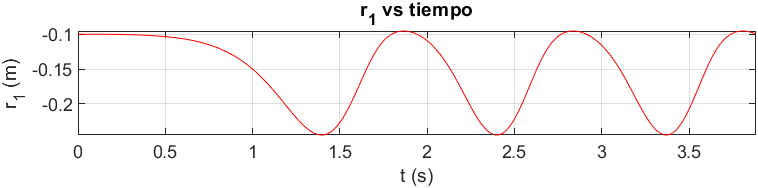
\includegraphics[width=8cm, height=12cm,keepaspectratio]{NR Simultaneo/r1.png}}
    \end{figure}
    \vspace{-25pt}
        \begin{figure} [H]
        \centerline{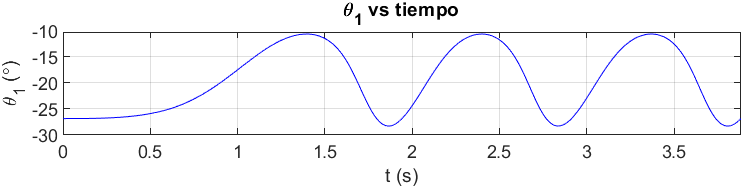
\includegraphics[width=8cm, height=12cm,keepaspectratio]{NR Simultaneo/theta1.png}}
    \end{figure}
        \vspace{-25pt}
        \begin{figure} [H]
        \centerline{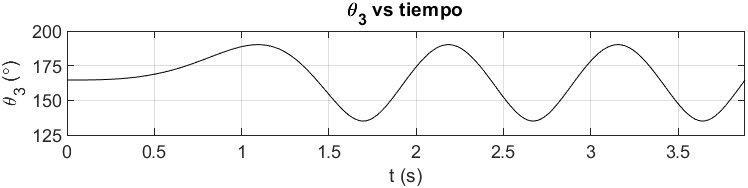
\includegraphics[width=8cm, height=12cm,keepaspectratio]{NR Simultaneo/theta3.png}}
        \caption{Posiciones para NR simultaneo.}
        \label{}
    \end{figure}
\begin{figure} [H]
        \centerline{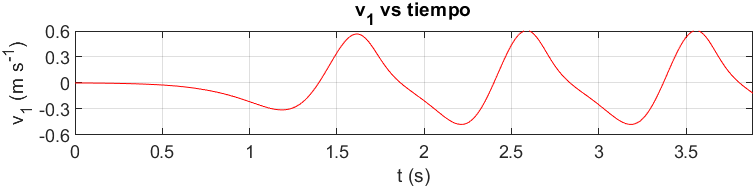
\includegraphics[width=8cm, height=12cm,keepaspectratio]{NR Simultaneo/v1.png}}
    \end{figure}
    \vspace{-25pt}
        \begin{figure} [H]
        \centerline{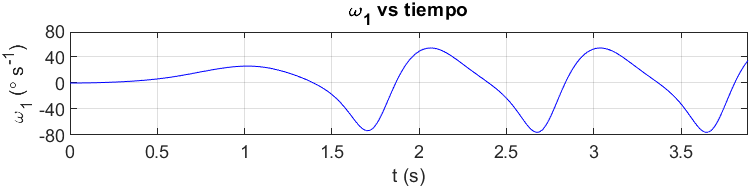
\includegraphics[width=8cm, height=12cm,keepaspectratio]{NR Simultaneo/w1.png}}
    \end{figure}
        \vspace{-25pt}
        \begin{figure} [H]
        \centerline{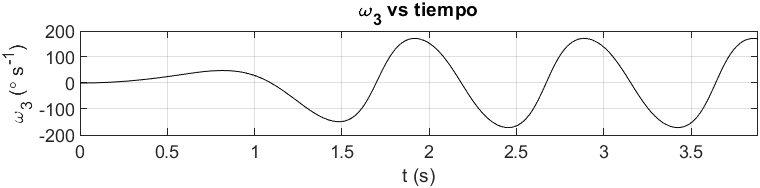
\includegraphics[width=8cm, height=12cm,keepaspectratio]{NR Simultaneo/w3.png}}
        \caption{Velocidades para NR simultaneo.}
        \label{}
    \end{figure}
\begin{figure} [H]
        \centerline{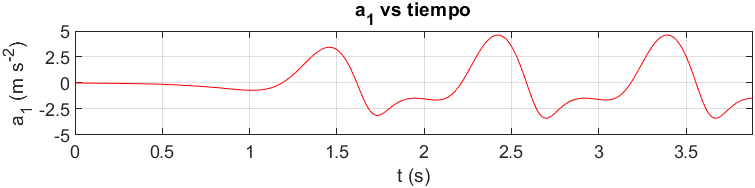
\includegraphics[width=8cm, height=12cm,keepaspectratio]{NR Simultaneo/a1.png}}
    \end{figure}
    \vspace{-25pt}
        \begin{figure} [H]
        \centerline{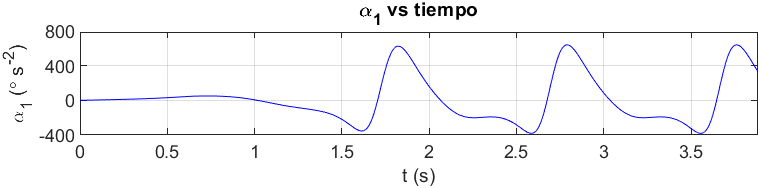
\includegraphics[width=8cm, height=12cm,keepaspectratio]{NR Simultaneo/alpha1.png}}
    \end{figure}
        \vspace{-25pt}
        \begin{figure} [H]
        \centerline{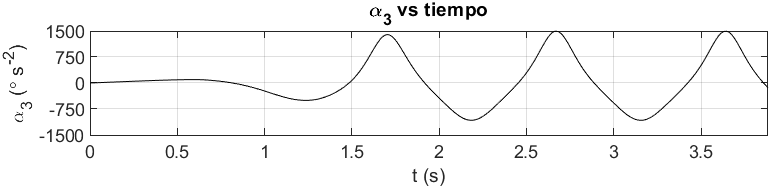
\includegraphics[width=8cm, height=12cm,keepaspectratio]{NR Simultaneo/alpha3.png}}
        \caption{Aceleraciones para NR simultaneo.}
        \label{}
    \end{figure}
        \begin{figure} [H]
        \centerline{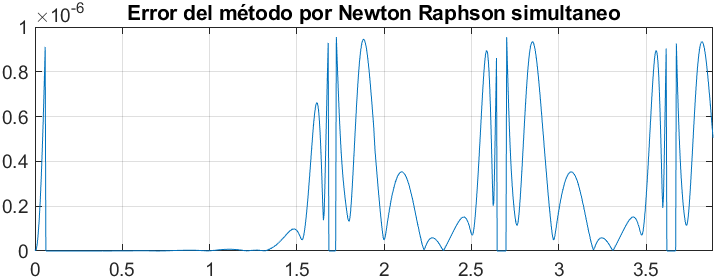
\includegraphics[width=8cm, height=12cm,keepaspectratio]{Implementacion/error Resultados NR.png}}
        \caption{Error asociado al método de NR simultáneo.}
        \label{ERRORNR}
    \end{figure}   
\end{multicols}
\subsection{NR Consecutivo}
El mismo procedimiento realizado para el método de Newton Raphson de forma simultanea se realiza para el método de forma consecutiva. Debido a la extensión del documento, y a la similitud que se tienen con los resultados anteriores, las gráficas de resultados se encuentran en el anexo \ref{NRconsecutivo}.
\subsection{Simulación}
Para poder corroborar los resultados obtenidos mediante el uso del método de Newton Raphson, se decide hacer un modelado 3D del mecanismo en el software \textit{Autodesk Inventor}. El mecanismo simulado resume el movimiento de la sierra eléctrica real utilizando eslabones y juntas que definidos a partir de las condiciones iniciales del problema.
\begin{figure} [H]
    \centerline{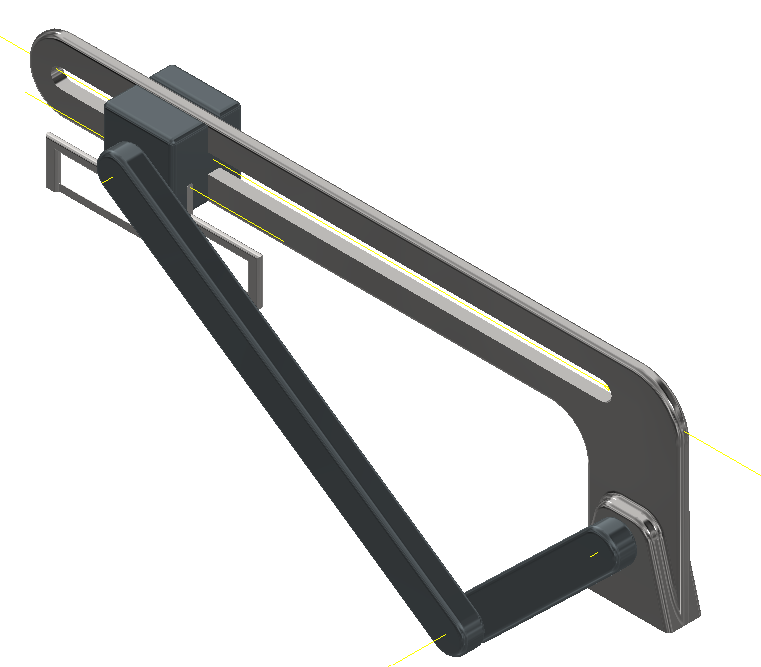
\includegraphics[width=8cm, height=6cm,keepaspectratio]{Mecanismo 3D .png}}
    \caption{Modelo en Inventor del Mecanismo 3D}
    \label{}
\end{figure}
Como se puede evidenciar, a la bancada se conecta la manivela, el cual es el eslabón donde se genera el movimiento por el perfil cinemático del motor. A la manivela se le conecta el acoplador, el cual es el eslabón de mayor extensión, también conectado a la corredera, la cual se une a la sierra y se pueden desplazar sobre la guía de la bancada.

Los resultados de simulación se generan a partir del entorno de simulación dinámica del software. En este entorno, se impone el perfil de velocidad del motor al eje de la manivela, donde es el mismo perfil utilizado para encontrar los resultados por NR. Con esto, se genera la simulación del modelado, donde se pueden extraer los valores cinemáticos de todas las variables implicadas en el sistema. Cabe resaltar que, al igual que con el método de NR, se resuelve para 1000 puntos en un periodo de $3.883\;s$. Las gráficas de resultados se encuentran en el anexo \ref{RInventor}.
\section{Análisis de resultados}
\subsection{Comparación de aplicación de NR}
Se realizaron dos variaciones del método de Newton Raphson, uno donde se resolvían las nueve variables en simultaneo, y otra donde se resolvían de manera consecutiva, por lo que es conveniente señalar las diferencias entre estos dos casos. Lo primero es comparar los errores asociados al método, comparando la figura \ref{ERRORNR} con la figura \ref{ERRORNREX} del anexo \ref{NRconsecutivo}, El error del método simultáneo suele ser mayor al método consecutivo, sin embargo, todos los valores están acotados por la tolerancia establecida $\varepsilon$. Ahora, se muestra el error absoluto entre estos dos casos:
\begin{figure} [H]
    \centerline{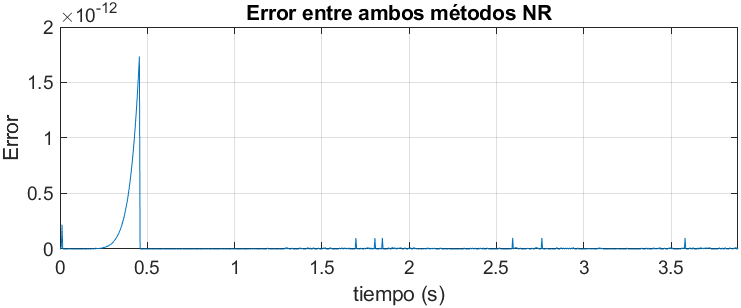
\includegraphics[width=8cm, height=12cm,keepaspectratio]{Implementacion/Error entre NR.png}}
    \caption{Error absoluto entre las versiones del método de Newton Raphson}
    \label{}
\end{figure}
Como se puede evidenciar, un error absoluto en el orden de $10^{-12}$ mientras se tiene una cota de error del método de $\varepsilon<10^{-6}$ indica que los resultados obtenidos entre los métodos fueron bastante precisos a pesar de resolverse de maneras distintas.

Ahora bien, para definir cual de estos dos se toma como la solución final del sistema, se va a mostrar el tiempo de ejecución para cada caso. De este modo, se puede establecer cual caso es más eficiente en calcular los resultados.
\begin{figure}[H]
\centering
  \begin{subfigure}[b]{0.49\textwidth}
    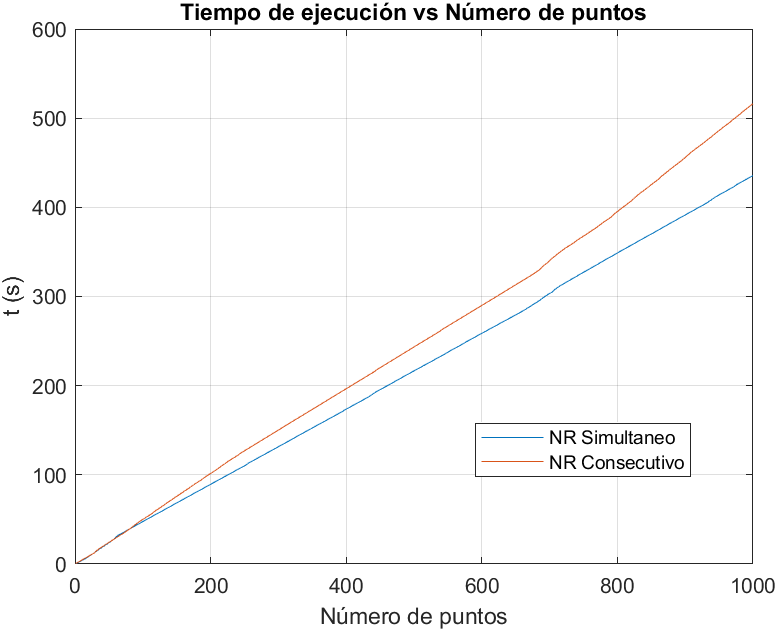
\includegraphics[width=7.5 cm, height=7.5 cm, keepaspectratio]{Implementacion/Dif tiempo ejecucion.png}
    \caption{Tiempo de ejecución para los métodos.}
    \label{}
  \end{subfigure}
  \hfill
  \begin{subfigure}[b]{0.49\textwidth}
    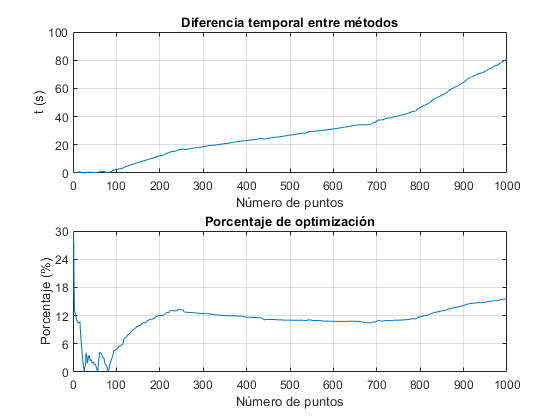
\includegraphics[width=8.5 cm, height=8.5 cm, keepaspectratio]{Implementacion/optimizacion tiempo.png}
    \caption{Diferencia en los tiempos de ejecución.}
    \label{}
  \end{subfigure}\\
  \vspace{10pt}
  \caption{Resultados de tiempo de ejecución del sistema.}
  \vspace{-10pt}
\end{figure}
Como se puede evidenciar, resolver el sistema mediante el método de Newton Raphson de manera simultánea es más óptimo que realizarlo de manera consecutiva. A pesar de que los tiempos de ejecución tienen un comportamiento lineal, la pendiente del método de forma consecutiva es más elevada. Dicho esto, considerando que los resultados obtenidos por ambos métodos son casi iguales, y que se tiene una reducción del tiempo de ejecución de aproximadamente $12\%$ para el método en simultáneo, este se considera como la mejor solución, teniendo en cuenta que ese porcentaje es considerablemente alto cuando se trabaja con un número de datos elevados. Así pues, se van a considerar los resultados obtenidos por el método de NR simultáneo como los resultados finales del problema. 
\subsection{Error absoluto del método de Newton Raphson}
A partir de las ecuaciones determinadas en la sección \ref{solAna} se pueden determinar las soluciones exactas del problema, donde se van a utilizar para determinar el error absoluto que se generó al solucionar el sistema. Al realizar este procedimiento, se determinan los siguientes errores absolutos a las soluciones encontradas.
\begin{multicols}{2}
\begin{figure} [H]
        \centerline{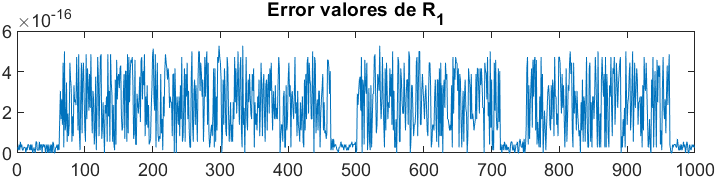
\includegraphics[width=8cm, height=12cm,keepaspectratio]{Error/Error R1.png}}
    \end{figure}
    \vspace{-25pt}
        \begin{figure} [H]
        \centerline{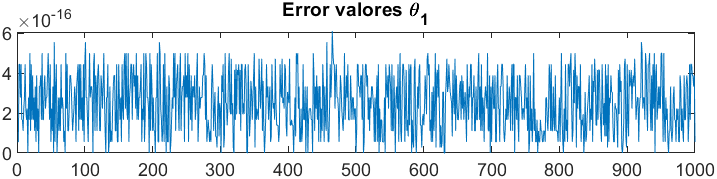
\includegraphics[width=8cm, height=12cm,keepaspectratio]{Error/Error theta1.png}}
    \end{figure}
        \vspace{-25pt}
        \begin{figure} [H]
        \centerline{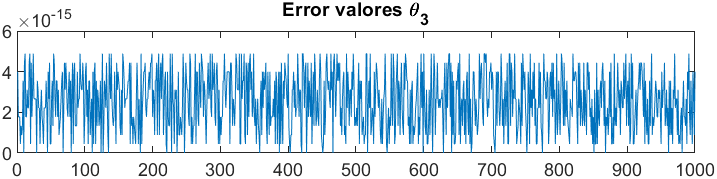
\includegraphics[width=8cm, height=12cm,keepaspectratio]{Error/Error theta3.png}}
        \caption{Error absoluto para resultados de posición.}
        \label{}
    \end{figure}
\begin{figure} [H]
        \centerline{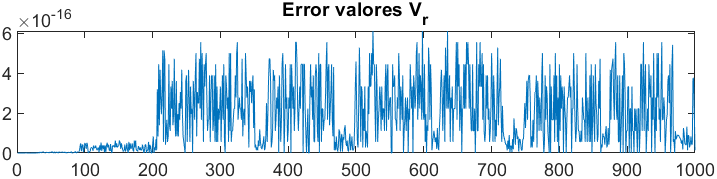
\includegraphics[width=8cm, height=12cm,keepaspectratio]{Error/Error Vr.png}}
    \end{figure}
    \vspace{-25pt}
        \begin{figure} [H]
        \centerline{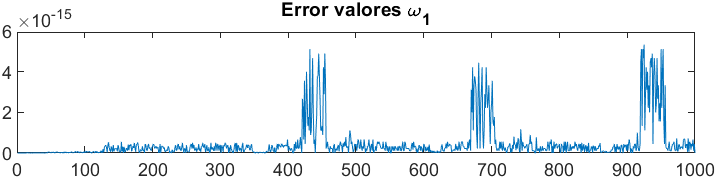
\includegraphics[width=8cm, height=12cm,keepaspectratio]{Error/Error omega1.png}}
    \end{figure}
        \vspace{-25pt}
        \begin{figure} [H]
        \centerline{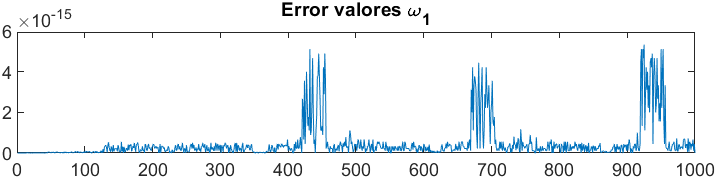
\includegraphics[width=8cm, height=12cm,keepaspectratio]{Error/Error omega1.png}}
        \caption{Error absoluto para resultados de velocidad.}
        \label{}
    \end{figure}
\end{multicols}
\begin{figure} [H]
        \centerline{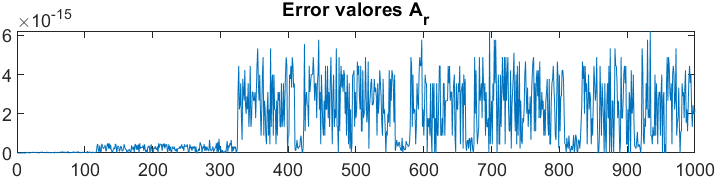
\includegraphics[width=8cm, height=12cm,keepaspectratio]{Error/Error Ar.png}}
    \end{figure}
    \vspace{-25pt}
        \begin{figure} [H]
        \centerline{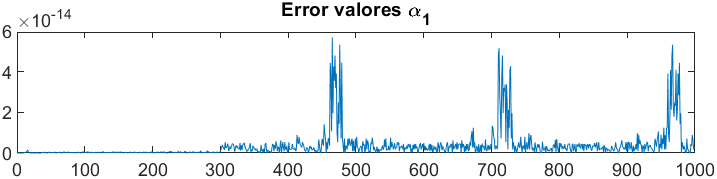
\includegraphics[width=8cm, height=12cm,keepaspectratio]{Error/Error alpha1.png}}
    \end{figure}
        \vspace{-25pt}
        \begin{figure} [H]
        \centerline{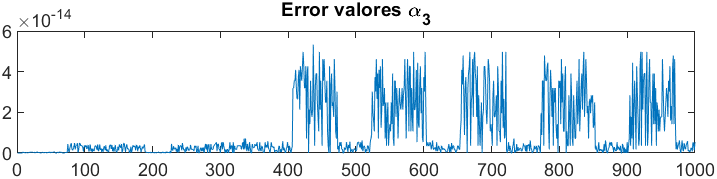
\includegraphics[width=8cm, height=12cm,keepaspectratio]{Error/Error alpha3.png}}
        \caption{Error absoluto para resultados de aceleración.}
        \label{}
    \end{figure}
Como se puede evidenciar en las gráficas, el error absoluto asociado a las posiciones y velocidades del sistema se encuentra en el orden de $10^{-15}$, mientras que para las aceleraciones se encuentra en el orden de $10^{-14}$. Ahora bien, teniendo en cuenta que el error de NR se acotó como $\varepsilon<10^{-6}$, y que el error absoluto de todos los resultados siempre es menor a $10^{-13}$, se establece que los valores obtenidos mediante el método de Newton Raphson simultaneo fueron altamente exactos y que resolver el sistema mediante esta versión del método numérico es una manera bastante sencilla y efectiva de solución.
\subsection{Comparación de resultados NR-Simulación \textit{Inventor}}
Para finalizar, se van a comparar los resultados obtenidos por el método de Newton Raphson con los valores de simulación que se pueden evidenciar en el anexo \ref{RInventor}. De este modo, los resultados de \textit{Inventor} se obtienen a partir de una interfaz de simulación dinámica altamente utilizada para resolver este tipo de sistemas en las aplicaciones de ingeniería, debido a su capacidad de mostrar de manera virtual el comportamiento de los mecanismos ensamblados en la vida real. Hecha esta observación, se superponen los resultados obtenidos para el sistema con los valores obtenidos en \textit{Inventor}, obteniendo las siguientes gráficas: 
\begin{multicols}{2}
\begin{figure} [H]
        \centerline{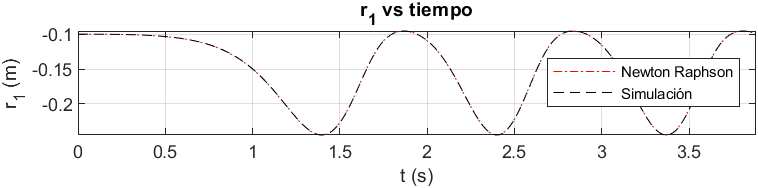
\includegraphics[width=8cm, height=12cm,keepaspectratio]{Inventor vs NR/r1 vs inventor.png}}
    \end{figure}
    \vspace{-25pt}
        \begin{figure} [H]
        \centerline{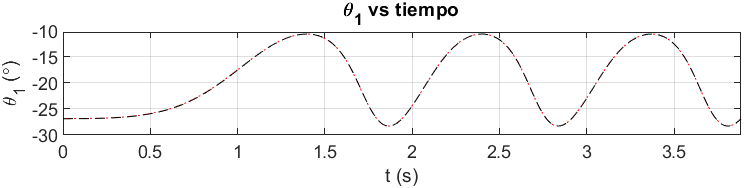
\includegraphics[width=8cm, height=12cm,keepaspectratio]{Inventor vs NR/theta1 vs inventor.png}}
    \end{figure}
        \vspace{-25pt}
        \begin{figure} [H]
        \centerline{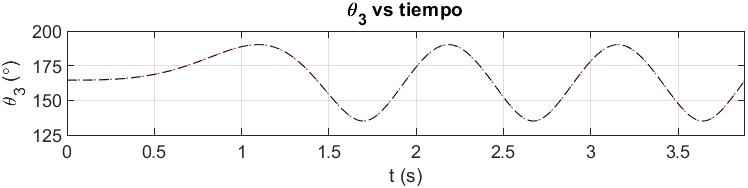
\includegraphics[width=8cm, height=12cm,keepaspectratio]{Inventor vs NR/theta3 vs inventor.png}}
        \caption{Comparación NR-Inventor para el perfil de posición.}
        \label{}
    \end{figure}
\begin{figure} [H]
        \centerline{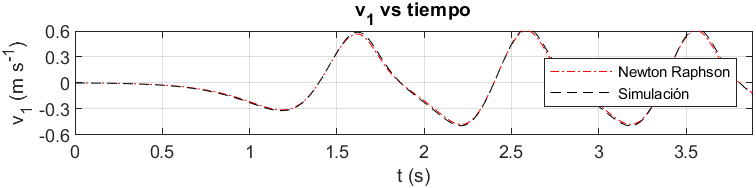
\includegraphics[width=8cm, height=12cm,keepaspectratio]{Inventor vs NR/v1 vs inventor.png}}
    \end{figure}
    \vspace{-25pt}
        \begin{figure} [H]
        \centerline{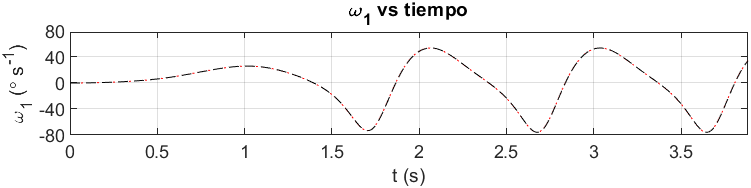
\includegraphics[width=8cm, height=12cm,keepaspectratio]{Inventor vs NR/w1 vs inventor.png}}
    \end{figure}
        \vspace{-25pt}
        \begin{figure} [H]
        \centerline{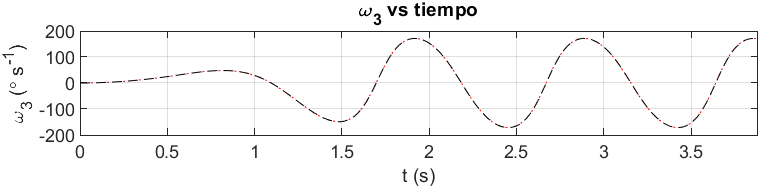
\includegraphics[width=8cm, height=12cm,keepaspectratio]{Inventor vs NR/w3 vs inventor.png}}
        \caption{Comparación NR-Inventor para el perfil de velocidad.}
        \label{}
    \end{figure}
\end{multicols}
\begin{figure} [H]
        \centerline{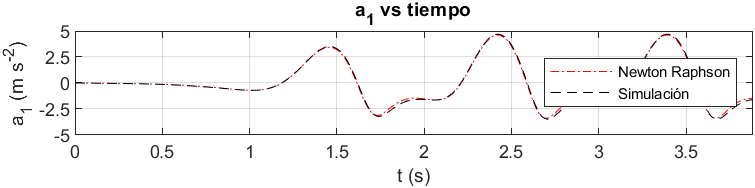
\includegraphics[width=8cm, height=12cm,keepaspectratio]{Inventor vs NR/a1 vs inventor.png}}
    \end{figure}
    \vspace{-25pt}
        \begin{figure} [H]
        \centerline{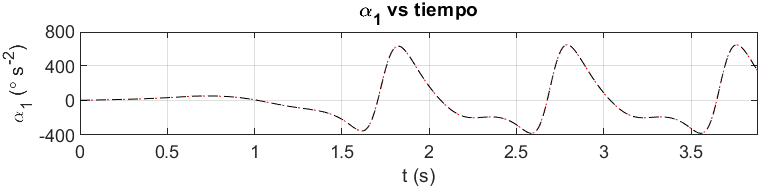
\includegraphics[width=8cm, height=12cm,keepaspectratio]{Inventor vs NR/alpha1 vs inventor.png}}
    \end{figure}
        \vspace{-25pt}
        \begin{figure} [H]
        \centerline{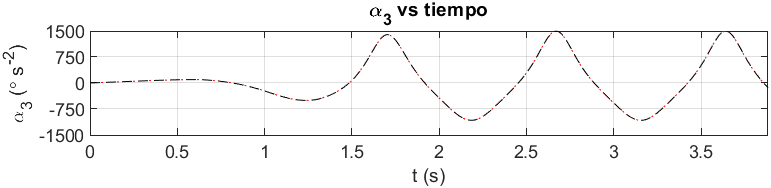
\includegraphics[width=8cm, height=12cm,keepaspectratio]{Inventor vs NR/alpha3 vs inventor.png}}
        \caption{Comparación NR-Inventor para el perfil de aceleración.}
        \label{}
    \end{figure}
Como es posible apreciar mediante el análisis de las gráficas, los resultados obtenidos en la simulación en \textit{Inventor} concuerdan con los valores obtenidos mediante el método de Newton Raphson simultaneo. Esto quiere decir que mediante la implementación de sistemas de solución por simulaciones CAD se obtienen resultados semejantes a los que se determinan resolviendo el mismo sistema utilizando el método numérico de Newton Raphson para sistemas de ecuaciones no lineales, con lo que se puede establecer la veracidad de solucionan del mecanismo a partir del método.
\section{Conclusiones}
\begin{itemize}
    \item Se puede implementar el método de Newton Raphson para resolver los sistemas de ecuaciones que describen problemas aplicados a la ingeniería, en este caso, los perfiles cinemáticos asociados a un mecanismo.
    \item El uso recurrente de métodos numéricos se puede implementar como procedimiento de solución a la cinemática de mecanismos para cualquier instante $t_0$ o intervalo $[t_0\;\;t_1]$, esto con el fin de optimizar la precisión de la solución y de los recursos computacionales asociados al mismo.
    \item Se obtienen los mismos resultados finales resolviendo mediante Newton Raphson el sistema de posición, velocidad y aceleración simultáneamente, a resolver cada uno de estos de manera individual. Además, resolver el mecanismo de manera simultánea reduce los recursos computacionales asociados a la solución, disminuyendo el tiempo total para solucionar el sistema.
    \item Se tiene una alta exactitud de solución al problema al implementar el método de Newton Raphson, obteniendo un error absoluto con la solución analítica menor a $10^{-13}$ para cualquier caso del sistema. Sumado a esto, al contrastar los resultados con las simulaciones del mecanismo en $Autodesk\;Inventor$, se logra establecer la veracidad de la solución para toda variable e instante del movimiento.
\end{itemize}
\section{Referencias}
\color{white}
\begin{thebibliography}{}
\vspace{-30pt}
\color{black}
\bibitem{mecanismo}Myzka,H,David.(2012).Máquinas y Mecanismos.4.Ed.
\bibitem{chapra}Chapra, S. C., \& Canale, R. P.  Numerical methods for engineers. McGraw-Hill Higher Education,  Boston, 2006
\bibitem{mathews}Mathews, J.H. \& Fink, K.D. Métodos numéricos con Matlab. Prentice Hall,  Madrid, 2000

\end{thebibliography}


\newpage
\color{black}
\appendix
\section{Gráficas de resultados para el método de Newton Raphson consecutivo} \label{NRconsecutivo}

\begin{multicols}{2}
\begin{figure} [H]
        \centerline{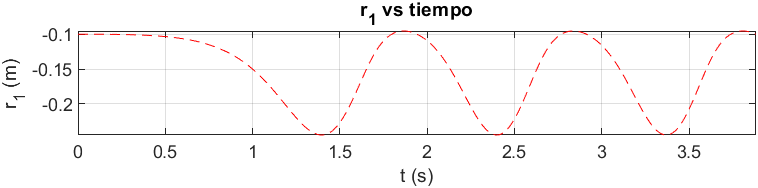
\includegraphics[width=8cm, height=12cm,keepaspectratio]{NR Consecutivo/r1.png}}
    \end{figure}
    \vspace{-20pt}
        \begin{figure} [H]
        \centerline{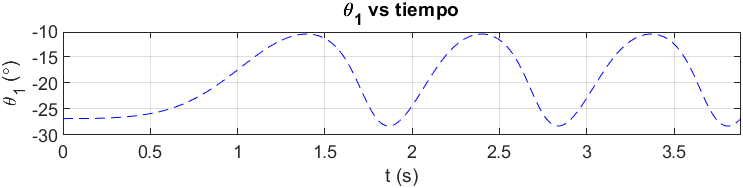
\includegraphics[width=8cm, height=12cm,keepaspectratio]{NR Consecutivo/theta1.png}}
    \end{figure}
        \vspace{-20pt}
        \begin{figure} [H]
        \centerline{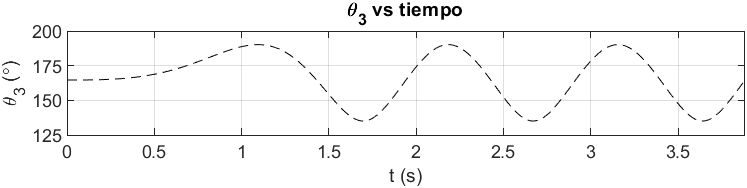
\includegraphics[width=8cm, height=12cm,keepaspectratio]{NR Consecutivo/theta3.png}}
        \caption{Posiciones para NR consecutivo.}
        \label{}
    \end{figure}
\begin{figure} [H]
        \centerline{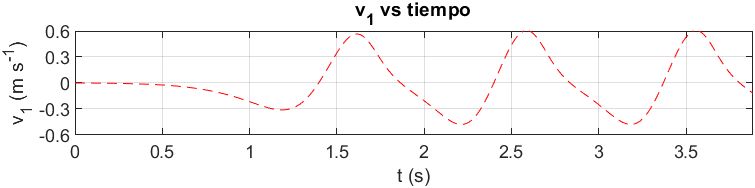
\includegraphics[width=8cm, height=12cm,keepaspectratio]{NR Consecutivo/v1.png}}
    \end{figure}
        \vspace{-20pt}
        \begin{figure} [H]
        \centerline{\includegraphics[width=8cm, height=12cm,keepaspectratio]{NR Consecutivo/w1.png}}
    \end{figure}
        \vspace{-20pt}
        \begin{figure} [H]
        \centerline{\includegraphics[width=8cm, height=12cm,keepaspectratio]{NR Consecutivo/w3.png}}
        \caption{Velocidades para NR consecutivo.}
        \label{}
    \end{figure}
\begin{figure} [H]
        \centerline{\includegraphics[width=8cm, height=12cm,keepaspectratio]{NR Consecutivo/a1.png}}
    \end{figure}
        \vspace{-20pt}
        \begin{figure} [H]
        \centerline{\includegraphics[width=8cm, height=12cm,keepaspectratio]{NR Consecutivo/alpha1.png}}
    \end{figure}
        \vspace{-20pt}
        \begin{figure} [H]
        \centerline{\includegraphics[width=8cm, height=12cm,keepaspectratio]{NR Consecutivo/alpha3.png}}
        \caption{Aceleraciones para NR consecutivo.}
        \label{}
    \end{figure}
        \begin{figure} [H]
        \centerline{\includegraphics[width=8cm, height=12cm,keepaspectratio]{Implementacion/error Resultados NR_EX.png}}
        \caption{Error asociado al método de NR consecutivo.}
        \label{ERRORNREX}
    \end{figure}   
\end{multicols} 

\newpage

\section{Resultados de simulación de inventor}\label{RInventor}

\begin{multicols}{2}
\begin{figure} [H]
        \centerline{\includegraphics[width=8cm, height=12cm,keepaspectratio]{simulacion/a2.png}}
    \end{figure}
    \vspace{-20pt}
        \begin{figure} [H]
        \centerline{\includegraphics[width=8cm, height=12cm,keepaspectratio]{simulacion/v2.png}}
    \end{figure}
        \vspace{-20pt}
        \begin{figure} [H]
        \centerline{\includegraphics[width=8cm, height=12cm,keepaspectratio]{simulacion/p2.png}}
        \caption{Perfil cinemático del eje del motor en \textit{Autodesk Inventor}.}
        \label{}
    \end{figure}
\begin{figure} [H]
        \centerline{\includegraphics[width=8cm, height=12cm,keepaspectratio]{simulacion/r1.png}}
    \end{figure}
        \vspace{-20pt}
        \begin{figure} [H]
        \centerline{\includegraphics[width=8cm, height=12cm,keepaspectratio]{simulacion/theta1.png}}
    \end{figure}
        \vspace{-20pt}
        \begin{figure} [H]
        \centerline{\includegraphics[width=8cm, height=12cm,keepaspectratio]{simulacion/theta3.png}}
        \caption{Posiciones obtenidas en \textit{Autodesk Inventor}}
        \label{}
    \end{figure}
\begin{figure} [H]
        \centerline{\includegraphics[width=8cm, height=12cm,keepaspectratio]{simulacion/vr.png}}
    \end{figure}
        \vspace{-20pt}
        \begin{figure} [H]
        \centerline{\includegraphics[width=8cm, height=12cm,keepaspectratio]{simulacion/omega1.png}}
    \end{figure}
        \vspace{-20pt}
        \begin{figure} [H]
        \centerline{\includegraphics[width=8cm, height=12cm,keepaspectratio]{simulacion/omega3.png}}
        \caption{Velocidades obtenidas en \textit{Autodesk Inventor}}
        \label{}
    \end{figure}
\begin{figure} [H]
        \centerline{\includegraphics[width=8cm, height=12cm,keepaspectratio]{simulacion/a1.png}}
    \end{figure}
        \vspace{-20pt}
        \begin{figure} [H]
        \centerline{\includegraphics[width=8cm, height=12cm,keepaspectratio]{simulacion/alpha1.png}}
    \end{figure}
        \vspace{-20pt}
        \begin{figure} [H]
        \centerline{\includegraphics[width=8cm, height=12cm,keepaspectratio]{simulacion/alpha3.png}}
        \caption{Aceleraciones obtenidas en \textit{Autodesk Inventor}.}
        \label{}
    \end{figure}    
\end{multicols} 

\newpage

\section{Jacobianos Inversos}
\subsection{Posición:}
\begin{equation*}
\begin{array}{l}
J^{-1}_{pos}=\left(\begin{array}{ccc}
\frac{1}{\mathrm{sin}\left(\theta_1 \right)} & -\frac{r_1 \,\mathrm{cos}\left(\theta_1 \right)}{r_{\textrm{1y}} \,\mathrm{sin}\left(\theta_1 \right)\,\sigma_1 } & \frac{r_1 \,\mathrm{cos}\left(\theta_1 \right)\,\mathrm{sin}\left(\theta_3 \right)}{r_{\textrm{1y}} \,\mathrm{cos}\left(\theta_3 \right)\,\mathrm{sin}\left(\theta_1 \right)\,\sigma_1 }\\
0 & \frac{1}{r_{\textrm{1y}} \,\sigma_1 } & -\frac{\mathrm{sin}\left(\theta_3 \right)}{r_{\textrm{1y}} \,\mathrm{cos}\left(\theta_3 \right)\,\sigma_1 }\\
0 & 0 & -\frac{1}{r_3 \,\mathrm{cos}\left(\theta_3 \right)}
\end{array}\right)\\
\mathrm{}\\
\textrm{Donde:}\\
\mathrm{}\\
\;\;\sigma_1 ={\mathrm{cot}\left(\theta_1 \right)}^2 +1
\end{array}
\label{jacobiano inv pos}    
\end{equation*}
\subsection{Velocidad:}
\begin{equation*}
\begin{array}{l}
J^{-1}_{vel}=\left(\begin{array}{ccc}
-\frac{\mathrm{cos}\left(\theta_1 \right)}{{\mathrm{cos}\left(\theta_1 \right)}^2 +{\mathrm{sin}\left(\theta_1 \right)}^2 } & \frac{\sigma_4 }{\sigma_2 } & -\frac{\sigma_4 -\mathrm{cos}\left(\theta_3 \right)\,\mathrm{sin}\left(\theta_1 \right)}{\sigma_2 }\\
\frac{\mathrm{sin}\left(\theta_1 \right)}{r_1 \,{\mathrm{cos}\left(\theta_1 \right)}^2 +r_1 \,{\mathrm{sin}\left(\theta_1 \right)}^2 } & -\frac{\sigma_3 }{\sigma_1 } & \frac{\mathrm{cos}\left(\theta_1 \right)\,\mathrm{cos}\left(\theta_3 \right)+\sigma_3 }{\sigma_1 }\\
0 & -\sigma_5  & \sigma_5 
\end{array}\right)\\
\mathrm{}\\
\textrm{Donde:}\\
\mathrm{}\\
\;\;\sigma_1 =r_1 \,\mathrm{cos}\left(\theta_3 \right)\,{\mathrm{cos}\left(\theta_1 \right)}^2 +r_1 \,\mathrm{cos}\left(\theta_3 \right)\,{\mathrm{sin}\left(\theta_1 \right)}^2 \\
\mathrm{}\\
\;\;\sigma_2 =\mathrm{cos}\left(\theta_3 \right)\,{\mathrm{cos}\left(\theta_1 \right)}^2 +\mathrm{cos}\left(\theta_3 \right)\,{\mathrm{sin}\left(\theta_1 \right)}^2 \\
\mathrm{}\\
\;\;\sigma_3 =\mathrm{sin}\left(\theta_1 \right)\,\mathrm{sin}\left(\theta_3 \right)\\
\mathrm{}\\
\;\;\sigma_4 =\mathrm{cos}\left(\theta_1 \right)\,\mathrm{sin}\left(\theta_3 \right)\\
\mathrm{}\\
\;\;\sigma_5 =\frac{1}{r_3 \,\mathrm{cos}\left(\theta_3 \right)}
\end{array}
\label{jacobiano inv vel}    
\end{equation*}
\subsection{Aceleración:}
\begin{equation*}
\begin{array}{l}
J_{ac}^{-1}=\left(\begin{array}{ccc}
-\frac{\sigma_4 -\mathrm{cos}\left(\theta_3 \right)\,\mathrm{sin}\left(\theta_1 \right)}{\sigma_2 } & -\frac{\mathrm{cos}\left(\theta_1 \right)}{{\mathrm{cos}\left(\theta_1 \right)}^2 +{\mathrm{sin}\left(\theta_1 \right)}^2 } & \frac{\sigma_4 }{\sigma_2 }\\
\frac{\mathrm{cos}\left(\theta_1 \right)\,\mathrm{cos}\left(\theta_3 \right)+\sigma_3 }{\sigma_1 } & \frac{\mathrm{sin}\left(\theta_1 \right)}{r_1 \,{\mathrm{cos}\left(\theta_1 \right)}^2 +r_1 \,{\mathrm{sin}\left(\theta_1 \right)}^2 } & -\frac{\sigma_3 }{\sigma_1 }\\
\sigma_5  & 0 & -\sigma_5 
\end{array}\right)\\
\mathrm{}\\
\textrm{Donde:}\\
\mathrm{}\\
\;\;\sigma_1 =r_1 \,\mathrm{cos}\left(\theta_3 \right)\,{\mathrm{cos}\left(\theta_1 \right)}^2 +r_1 \,\mathrm{cos}\left(\theta_3 \right)\,{\mathrm{sin}\left(\theta_1 \right)}^2 \\
\mathrm{}\\
\;\;\sigma_2 =\mathrm{cos}\left(\theta_3 \right)\,{\mathrm{cos}\left(\theta_1 \right)}^2 +\mathrm{cos}\left(\theta_3 \right)\,{\mathrm{sin}\left(\theta_1 \right)}^2 \\
\mathrm{}\\
\;\;\sigma_3 =\mathrm{sin}\left(\theta_1 \right)\,\mathrm{sin}\left(\theta_3 \right)\\
\mathrm{}\\
\;\;\sigma_4 =\mathrm{cos}\left(\theta_1 \right)\,\mathrm{sin}\left(\theta_3 \right)\\
\mathrm{}\\
\;\;\sigma_5 =\frac{1}{r_3 \,\mathrm{cos}\left(\theta_3 \right)}
\end{array}
    \label{jacobiano inv ac}
\end{equation*}
\newpage
\section{Jacobiano del sistema simultaneo:}\label{JAC9}
\small
\begin{turn}{90}
\begin{equation*}
\begin{array}{cc}
\mathrm{\textbf{Col. 1-3:}}&\\
&\left(\begin{array}{cccc}
\mathrm{sin}\left(\theta_1 \right) & r_1 \,\mathrm{cos}\left(\theta_1 \right) & 0 \\
0 & r_{\textrm{1y}} \,{\left({\mathrm{cot}\left(\theta_1 \right)}^2 +1\right)} & \sigma_4 \\
0 & 0 & \sigma_5 \\
\omega_1 \,\mathrm{sin}\left(\theta_1 \right) & V_r \,\mathrm{sin}\left(\theta_1 \right)+\omega_1 \,r_1 \,\mathrm{cos}\left(\theta_1 \right) & -\omega_3 \,r_3 \,\mathrm{cos}\left(\theta_3 \right)\\
\omega_1 \,\mathrm{cos}\left(\theta_1 \right) & \sigma_6  & \omega_3 \,r_3 \,\mathrm{sin}\left(\theta_3 \right)\\
\omega_1 \,\mathrm{cos}\left(\theta_1 \right) & \sigma_6  & 0 \\
\sigma_3  & \sigma_1  & 0 \\
\mathrm{cos}\left(\theta_1 \right)\,{\omega_1 }^2 +\alpha_1 \,\mathrm{sin}\left(\theta_1 \right) & -r_1 \,\mathrm{sin}\left(\theta_1 \right)\,{\omega_1 }^2 +2\,V_r \,\mathrm{cos}\left(\theta_1 \right)\,\omega_1 +a_r \,\mathrm{sin}\left(\theta_1 \right)+\alpha_1 \,r_1 \,\mathrm{cos}\left(\theta_1 \right) & {\omega_3 }^2 \,r_3 \,\mathrm{sin}\left(\theta_3 \right)-\alpha_3 \,r_3 \,\mathrm{cos}\left(\theta_3 \right) \\
\sigma_3  & \sigma_1  & r_3 \,\mathrm{cos}\left(\theta_3 \right)\,{\omega_3 }^2 +\alpha_3 \,r_3 \,\mathrm{sin}\left(\theta_3 \right) 
\end{array}\right)
\end{array}
\end{equation*}
\end{turn}
\begin{turn}{90}
\begin{equation*}
\begin{array}{cc}
\mathrm{\textbf{Col. 4-6:}}&\\
&\left(\begin{array}{ccc}
 0 & 0 & 0 \\
0 & 0 & 0\\
0 & 0 & 0\\
-\mathrm{cos}\left(\theta_1 \right) & r_1 \,\mathrm{sin}\left(\theta_1 \right) & \sigma_4 \\
\mathrm{sin}\left(\theta_1 \right) & r_1 \,\mathrm{cos}\left(\theta_1 \right) & \sigma_5 \\
\mathrm{sin}\left(\theta_1 \right) & r_1 \,\mathrm{cos}\left(\theta_1 \right) & 0 \\
\sigma_7  & \sigma_2  & 0 \\
2\,\omega_1 \,\mathrm{sin}\left(\theta_1 \right) & 2\,V_r \,\mathrm{sin}\left(\theta_1 \right)+2\,\omega_1 \,r_1 \,\mathrm{cos}\left(\theta_1 \right) & -2\,\omega_3 \,r_3 \,\mathrm{cos}\left(\theta_3 \right) \\
\sigma_7  & \sigma_2  & 2\,\omega_3 \,r_3 \,\mathrm{sin}\left(\theta_3 \right) 
\end{array}\right)\\
\end{array}
\end{equation*}
\end{turn}
\begin{turn}{90}
\begin{equation*}
\begin{array}{cc}
\mathrm{\textbf{Col. 7-9:}}&\\
&\left(\begin{array}{ccc}
0 & 0 & 0\\
0 & 0 & 0\\
0 & 0 & 0\\
0 & 0 & 0\\
0 & 0 & 0\\
0 & 0 & 0\\
\sigma_7  & \,\mathrm{cos}\left(\theta_1 \right) & 0\\
-\mathrm{cos}\left(\theta_1 \right) & r_1 \,\mathrm{sin}\left(\theta_1 \right) & \sigma_4 \\
\mathrm{sin}\left(\theta_1 \right) & r_1 \,\mathrm{cos}\left(\theta_1 \right) & \sigma_5 
\end{array}\right)\\
\end{array}
\end{equation*}
\end{turn}
\newpage
\normalsize
\begin{equation*}
\mathrm{}\\
\begin{array}{l}
\textrm{Donde:}\\
\mathrm{}\\
\;\;\sigma_1 =-r_1 \,\mathrm{cos}\left(\theta_1 \right)\,{\omega_1 }^2 -2\,V_r \,\mathrm{sin}\left(\theta_1 \right)\,\omega_1 +a_r \,\mathrm{cos}\left(\theta_1 \right)-\alpha_1 \,r_1 \,\mathrm{sin}\left(\theta_1 \right)\\
\mathrm{}\\
\;\;\sigma_2 =2\,V_r \,\mathrm{cos}\left(\theta_1 \right)-2\,\omega_1 \,r_1 \,\mathrm{sin}\left(\theta_1 \right)\\
\mathrm{}\\
\;\;\sigma_3 =\alpha_1 \,\mathrm{cos}\left(\theta_1 \right)-{\omega_1 }^2 \,\mathrm{sin}\left(\theta_1 \right)\\
\mathrm{}\\
\;\;\sigma_4 =-r_3 \,\mathrm{sin}\left(\theta_3 \right)\\
\mathrm{}\\
\;\;\sigma_5 =-r_3 \,\mathrm{cos}\left(\theta_3 \right)\\
\mathrm{}\\
\;\;\sigma_6 =V_r \,\mathrm{cos}\left(\theta_1 \right)-\omega_1 \,r_1 \,\mathrm{sin}\left(\theta_1 \right)\\
\mathrm{}\\
\;\;\sigma_7 =2\,\omega_1 \,\mathrm{cos}\left(\theta_1 \right)
\end{array}
\end{equation*}
\newpage

\section{Códigos de Matlab del desarrollo}
A continuación se expone el listado de códigos generados para la solución del proyecto y la función que estos realizan:
\begin{enumerate}
    \item \textbf{Perfil cinemático:} Enfocado en la realización del perfil cinemático del motor, el cual se utiliza como datos de entrada al sistema.
    
    \item \textbf{Solución por Newton Raphson consecutivo:} Solución para un único punto para el método de Newton Raphson solucionando la posición, velocidad y aceleración de manera consecutiva. 
    \item \textbf{Solución por Newton Raphson simultáneo:} Solución para un único punto para el método de Newton Raphson solucionando la posición, velocidad y aceleración de manera simultánea.
    
    \item \textbf{Solución por método de Newton Raphson:} Solución a todo el perfil cinemático del motor para el mecanismo. Se implementan ambas versiones del NR y se comparan entre si.
    
    \item\textbf{ Solución analítica:} Se realiza la solución analítica para todo el perfil cinemático del motor para el mecanismo.
    
    \item \textbf{Resultados NR simultáneo vs solución analítica:} Comparar los resultados obtenidos por el método de NR con la solución analítica.
    
    \item \textbf{Resultados NR simultáneo vs simulación:} Comparar los resultados obtenidos por el método de NR con los resultados de simulación.
\end{enumerate}
Cabe resaltar que la mayoría de archivos utilizan datos externos en formato .txt, generados por los mismos u otro archivo de Matlab, por lo que es importante verificar la ruta de acceso a estos archivos.

\newpage
\subsection{Perfil cinemático}
\begin{lstlisting}
clear
clc
syms a1(t) a2(t) a3(t) a4(t) a5(t)  T A
syms v1(t) v2(t) v3(t) v4(t) v5(t)  
syms x1(t) x2(t) x3(t) x4(t) x5(t) 
assume(T>0)
assume(A>0)

A=5;

§\textrm{\large \textbf{Aceleracion}}§
a1(t)=3*A/T*t;
a2(t)=A;
a3(t)=-3*A/T*t;
Ca3=A-a3(2*T/3);
a3(t)=a3(t)+Ca3;
a4(t)=0;
fprintf('Funcion de aceleracion:')
aceleracion(t)=piecewise((0<=t<T/3),a1,(T/3<=t<2*T/3),a2,(2*T/3<=t<T),a3,(T<=t),a4)

§\textrm{\large \textbf{Velocidad}}§
v1(t)=int(a1);
v2(t)=int(a2);
Cv2=v1(T/3)-v2(T/3);
v2(t)=v2(t)+Cv2;
v3(t)=int(a3);
Cv3=v2(2*T/3)-v3(2*T/3);
v3(t)=v3(t)+Cv3;
v4(t)=int(a4);
Cv4=v3(T)-v4(T);
v4(t)=v4(t)+Cv4;
fprintf('Funcion de velocidad:')
velocidad(t)=piecewise((0<=t<T/3),v1,(T/3<=t<2*T/3),v2,(2*T/3<=t<T),v3,(t>=T),v4)

§\textrm{\large \textbf{Desplazamiento}}§
z1(t)=int(v1);
z2(t)=int(v2);
Cz2=z1(T/3)-z2(T/3);
z2(t)=z2(t)+Cz2;
z3(t)=int(v3);
Cz3=z2(2*T/3)-z3(2*T/3);
z3(t)=z3(t)+Cz3;
z4(t)=int(v4);
Cz4=z3(T)-z4(T);
z4(t)=z4(t)+Cz4;
fprintf('Funcion de desplazamiento:')
posicion(t)=piecewise((0<=t<T/3),z1,(T/3<=t<2*T/3),z2,(2*T/3<=t<T),z3,(t>=T),z4)

§\textrm{\large \textbf{Solucion de tMax}}§
f=2*pi==posicion(T);
Tgiro=solve(f,T);
aceleracion=subs(aceleracion,T,Tgiro);
velocidad=subs(velocidad,T,Tgiro);
posicion=subs(posicion,T,Tgiro);
fprintf('Tiempo de primera vuelta %.3f s',Tgiro)

§\textrm{\large \textbf{Graficas}}§
ts=linspace(0,2*Tgiro,1000);
Vmax=double(velocidad(Tgiro));

subplot(3,1,1)
plot(ts,aceleracion(ts))
title('Aceleracion angular vs tiempo')
grid on
xlabel('t (s)')
ylabel('\alpha (rad s^{-2})')
ylim([0 6])
xlim([0 double(2*Tgiro)])
yticks(0:2:6)

subplot(3,1,2)
plot(ts,velocidad(ts))
title('Velocidad angular vs tiempo')
grid on
xlabel('t (s)')
ylabel('\omega (rad s^{-1})')
ylim([0 Vmax*1.1])
xlim([0 double(2*Tgiro)])
yticks(0:2:8)

subplot(3,1,3)
plot(ts,posicion(ts))
title('Posicion angular vs tiempo')
grid on
xlabel('t (s)')
ylabel('\theta (rad)')
xlim([0 double(2*Tgiro)])
yticks(0:5:20)

TablaCinematica=table(double(ts)',double(aceleracion(ts))',double...
(velocidad(ts))',double(posicion(ts))');
TablaCinematica.Properties.VariableNames=["Tiempo","Aceleracion",...
"Velocidad","Posicion"]
writetable(TablaCinematica,'Perfil_cinematica.txt','delimiter',' ', 'WriteVariableNames', true)
TablaTXT=table(double(ts)',double(velocidad(ts)*180/pi)');
writetable(TablaTXT,'Perfil_Velocidad.txt','delimiter',' ', 'WriteVariableNames', false)
\end{lstlisting}
\newpage
\subsection{Solución por Newton  Raphson Consecutivo}
\begin{lstlisting}
clear
syms t Theta_1(t) Theta_2(t) Theta_3(t) R_1(t)
syms r_1 r_1y r_2 r_3 x
syms V_r omega_1 omega_2 omega_3 theta_1 theta_2 theta_3 
syms a_r alpha_1 alpha_2 alpha_3

§\textrm{\large \textbf{Ecuaciones}}§
Vr_2=0.075
Vr_3=0.17
Vr_1y=0.045

Vtheta_2=0
Vomega_2=0
Valpha_2=0

Fc=sin(Theta_1)*R_1-r_1y;
Fc=simplify(Fc,'Steps',5)

fc=subs(Fc,[Theta_1, R_1],[theta_1, r_1]);
SolR_1=solve(fc,r_1);

Fx=-R_1*cos(Theta_1)+r_2*cos(Theta_2)+r_3*cos(Theta_3);
Fx=simplify(Fx,'Steps',5)

fx=formula(subs(Fx,[Theta_1, Theta_2, Theta_3, R_1],[theta_1, theta_2, theta_3, SolR_1]))
fx=simplify(fx,'Steps',5)
SolTheta_1=solve(fx,theta_1);


Fy=R_1*sin(Theta_1)-r_2*sin(Theta_2)-r_3*sin(Theta_3);
Fy=simplify(Fy,'Steps',5)

fy=formula(subs(Fy,[Theta_1, Theta_2, Theta_3, R_1],[theta_1, theta_2, theta_3, SolR_1]))

SolTheta_3=solve(fy,theta_3);
SolTheta_3=SolTheta_3(1)

DFcDt=diff(Fc);
DFxDt=diff(Fx);
DFyDt=diff(Fy);

F1=formula(subs(DFxDt,[diff(R_1),diff(Theta_1),diff(Theta_2), ...
    diff(Theta_3),Theta_1,Theta_2,Theta_3,R_1],[V_r,omega_1,omega_2, ...
    omega_3,theta_1,theta_2,theta_3,r_1]))
F2=formula(subs(DFyDt,[diff(R_1),diff(Theta_1),diff(Theta_2), ...
    diff(Theta_3),Theta_1,Theta_2,Theta_3,R_1],[V_r,omega_1,omega_2, ...
    omega_3,theta_1,theta_2,theta_3,r_1]))
F3=formula(subs(DFcDt,[diff(R_1),diff(Theta_1),diff(Theta_2), ...
    diff(Theta_3),Theta_1,Theta_2,Theta_3,R_1],[V_r,omega_1,omega_2, ...
    omega_3,theta_1,theta_2,theta_3,r_1]))


D2FcDt2=diff(DFcDt);
D2FxDt2=diff(DFxDt);
D2FyDt2=diff(DFyDt);

F4=formula(subs(D2FcDt2,[diff(diff(R_1)),diff(diff(Theta_1)), ...
    diff(diff(Theta_2)),diff(diff(Theta_3)),diff(R_1),diff(Theta_1), ...
    diff(Theta_2),diff(Theta_3),Theta_1,Theta_2,Theta_3,R_1],[a_r, ...
    alpha_1,alpha_2,alpha_3,V_r,omega_1,omega_2,omega_3,theta_1, ...
    theta_2,theta_3,r_1]))
F5=formula(subs(D2FxDt2,[diff(diff(R_1)),diff(diff(Theta_1)), ...
    diff(diff(Theta_2)),diff(diff(Theta_3)),diff(R_1),diff(Theta_1), ...
    diff(Theta_2),diff(Theta_3),Theta_1,Theta_2,Theta_3,R_1],[a_r, ...
    alpha_1,alpha_2,alpha_3,V_r,omega_1,omega_2,omega_3,theta_1, ...
    theta_2,theta_3,r_1]))
F6=formula(subs(D2FyDt2,[diff(diff(R_1)),diff(diff(Theta_1)), ...
    diff(diff(Theta_2)),diff(diff(Theta_3)),diff(R_1),diff(Theta_1), ...
    diff(Theta_2),diff(Theta_3),Theta_1,Theta_2,Theta_3,R_1],[a_r, ...
    alpha_1,alpha_2,alpha_3,V_r,omega_1,omega_2,omega_3,theta_1, ...
    theta_2,theta_3,r_1]))

Pi=[-0.1,-0.5,3,-0.5,0,0.5,-0.5,0,0.5]
%Pi=[-0.0997,-0.4684,2.8737,0,0,0,0,0,0];

§\textrm{\large \textbf{Posición}}§

fP(r_1,theta_1,theta_3)=[fc;fx;fy];
fP=subs(fP,[theta_2,r_1y,r_2,r_3],[Vtheta_2,Vr_1y,Vr_2,Vr_3]);
fP=simplify(fP,'Steps',5);

valTheta_3=subs(SolTheta_3,[theta_2,r_2,r_3,r_1y],[Vtheta_2,Vr_2,Vr_3,Vr_1y]);
ValTheta_1=subs(SolTheta_1,[theta_2,r_2,r_3,r_1y,theta_3],[Vtheta_2,Vr_2, ...
    Vr_3,Vr_1y,valTheta_3]);
valR_1=subs(SolR_1,[r_1y,theta_1],[Vr_1y,ValTheta_1]);

JacP=jacobian(fP, [r_1,theta_1,theta_3]);
JacInvP=JacP^-1;


pP=[Pi(1),Pi(2),Pi(3)]';
ValoresPNR(1,:)=pP';
iteraciones=15;
for i=1:iteraciones
    pP=double(pP-JacInvP(pP(1),pP(2),pP(3))*fP(pP(1),pP(2),pP(3)));
    ValoresPNR(i+1,:)=double(pP)';
    ErrorNRP(i,:)=abs(ValoresPNR(i,:)-ValoresPNR(i+1,:));
    NormErrorNRP(i)=norm(ErrorNRP(i,:));
     if NormErrorNRP(i)<0.000001
        break;
    end
end
SolPosNR=double(pP);


§\textrm{\large \textbf{Velocidad}}§
fV(V_r,omega_1,omega_3)=[F1;F2;F3];
fV=subs(fV,[theta_2,r_1y,r_2,r_3,r_1,theta_1,theta_3,omega_2],[Vtheta_2, ...
    Vr_1y,Vr_2,Vr_3,SolPosNR(1),SolPosNR(2),SolPosNR(3),Vomega_2]);
fV=simplify(fV,'Steps',5);

JacV=jacobian(fV, [V_r,omega_1,omega_3]);
JacInvV=JacV^-1;

pV=[Pi(4),Pi(5),Pi(6)]';
ValoresVNR(1,:)=pV';

iteraciones=15;
for i=1:iteraciones
    pV=double(pV-JacInvV(pV(1),pV(2),pV(3))*fV(pV(1),pV(2),pV(3)));
    ValoresVNR(i+1,:)=double(pV)';
    ErrorNRV(i,:)=abs(ValoresVNR(i,:)-ValoresVNR(i+1,:));
    NormErrorNRV(i)=norm(ErrorNRV(i,:));
     if NormErrorNRV(i)<0.000001
        break;
    end
end

SolVelNR=double(pV);

§\textrm{\large \textbf{Aceleración}}§
fA(a_r,alpha_1,alpha_3)=[F4;F5;F6];
fA=subs(fA,[theta_2,r_1y,r_2,r_3,r_1,theta_1,theta_3,omega_2,V_r,omega_1, ...
    omega_3,alpha_2],[Vtheta_2,Vr_1y,Vr_2,Vr_3,SolPosNR(1),SolPosNR(2), ...
    SolPosNR(3),Vomega_2,SolVelNR(1),SolVelNR(2),SolVelNR(3),Valpha_2]);
fA=simplify(fA,'Steps',5);
JacA=jacobian(fA, [a_r,alpha_1,alpha_3]);
JacInvA=JacA^-1;

PiA=[Pi(7),Pi(8),Pi(9)]';
ValoresANR(1,:)=PiA';

iteraciones=15;
for i=1:iteraciones
    PiA=double(PiA-JacInvA(PiA(1),PiA(2),PiA(3))*fA(PiA(1),PiA(2),PiA(3)));
    ValoresANR(i+1,:)=double(PiA)';
    ErrorNRA(i,:)=abs(ValoresANR(i,:)-ValoresANR(i+1,:));
    NormErrorNRA(i)=norm(ErrorNRA(i,:));
     if NormErrorNRP(i)<0.000001
        break;
    end
end
SolAceNR=double(PiA);

§\textrm{\large \textbf{Gráficas}}§

figure()
plot(0:(length(ValoresPNR(:,1))-1),ValoresPNR)
title('Solucion posicion metodo de Newton Raphson')
legend("r_1","\theta_1","\theta_3","Location","best")
ylabel('Solucion')
xlabel('Indice')
xticks(0:length(ValoresPNR(:,1)))
grid on

figure()
subplot(2,1,1)
plot(ErrorNRP)
title('Error de posicion metodo de Newton Raphson')
legend("r_1","\theta_1","\theta_3","Location","best")
ylabel('Error')
xlabel('Iteraciones')
xticks(1:(length(ValoresPNR(:,1))-1))
grid on
subplot(2,1,2)
plot(NormErrorNRP)
title('Error total posicion metodo de Newton Raphson')
xlabel('Iteraciones')
xticks(1:(length(ValoresPNR(:,1))-1))
grid on


figure()
plot(0:(length(ValoresVNR(:,1))-1),ValoresVNR)
title('Solucion velocidad metodo de Newton Raphson')
legend("V_r","\omega_1","\omega_3","Location","best")
ylabel('Solucion')
xlabel('Indice')
xticks(0:length(ValoresVNR(:,1)))
grid on


figure()
subplot(2,1,1)
plot(ErrorNRV)
title('Error de velocidad metodo de Newton Raphson')
legend("V_r","\omega_1","\omega_3","Location","best")
ylabel('Error')
xlabel('Iteraciones')
xticks(1:(length(ValoresVNR(:,1))-1))
grid on
subplot(2,1,2)
plot(NormErrorNRV)
title('Error total velocidad metodo de Newton Raphson')
xlabel('Iteraciones')
xticks(1:(length(ValoresVNR(:,1))-1))
grid on

figure()
plot(0:(length(ValoresANR(:,1))-1),ValoresANR)
title('Solucion aceleracion metodo de Newton Raphson')
legend("a_r","\alpha_1","\alpha_3","Location","best")
ylabel('Solucion')
xlabel('Indice')
xticks(0:length(ValoresANR(:,1)))
grid on

figure()
subplot(2,1,1)
plot(ErrorNRA)
title('Error de aceleracion metodo de Newton Raphson')
legend("a_r","\alpha_1","\alpha_3","Location","best")
ylabel('Error')
xlabel('Iteraciones')
xticks(1:(length(ValoresANR(:,1))-1))
grid on
subplot(2,1,2)
plot(NormErrorNRA)
title('Error total aceleracion metodo de Newton Raphson')
xlabel('Iteraciones')
xticks(1:(length(ValoresANR(:,1))-1))
grid on

format long
Solucion=[SolPosNR;SolVelNR;SolAceNR]
\end{lstlisting}
\newpage
\subsection{Solución por Newton Raphson simultaneo}
\begin{lstlisting}
clear
clc
syms t Theta_1(t) Theta_2(t) Theta_3(t) R_1(t)


syms r_1 r_1y r_2 r_3 x

syms V_r omega_1 omega_2 omega_3 theta_1 theta_2 theta_3 

syms a_r alpha_1 alpha_2 alpha_3

Vr_2=0.075
Vr_3=0.17
Vr_1y=0.045

Vtheta_2=0
Vomega_2=0
Valpha_2=0

Fc=sin(Theta_1)*R_1-r_1y;
Fc=simplify(Fc,'Steps',5)
fc=subs(Fc,[Theta_1, R_1],[theta_1, r_1])
SolR_1=solve(fc,r_1)
Fx=-R_1*cos(Theta_1)+r_2*cos(Theta_2)+r_3*cos(Theta_3);
Fx=simplify(Fx,'Steps',5)
fx=formula(subs(Fx,[Theta_1, Theta_2, Theta_3, R_1],[theta_1, theta_2, theta_3, SolR_1]))
fx=simplify(fx,'Steps',5)
SolTheta_1=solve(fx,theta_1);
Fy=R_1*sin(Theta_1)-r_2*sin(Theta_2)-r_3*sin(Theta_3);
Fy=simplify(Fy,'Steps',5);
fy=formula(subs(Fy,[Theta_1, Theta_2, Theta_3, R_1],[theta_1, theta_2, theta_3, SolR_1]))
SolTheta_3=solve(fy,theta_3);
SolTheta_3=SolTheta_3(1);

DFcDt=diff(Fc);
DFxDt=diff(Fx);
DFyDt=diff(Fy);

F1=formula(subs(DFxDt,[diff(R_1),diff(Theta_1),diff(Theta_2), ...
    diff(Theta_3),Theta_1,Theta_2,Theta_3,R_1],[V_r,omega_1,omega_2, ...
    omega_3,theta_1,theta_2,theta_3,r_1]))
F2=formula(subs(DFyDt,[diff(R_1),diff(Theta_1),diff(Theta_2), ...
    diff(Theta_3),Theta_1,Theta_2,Theta_3,R_1],[V_r,omega_1,omega_2, ...
    omega_3,theta_1,theta_2,theta_3,r_1]))
F3=formula(subs(DFcDt,[diff(R_1),diff(Theta_1),diff(Theta_2), ...
    diff(Theta_3),Theta_1,Theta_2,Theta_3,R_1],[V_r,omega_1,omega_2, ...
    omega_3,theta_1,theta_2,theta_3,r_1]))


D2FcDt2=diff(DFcDt);
D2FxDt2=diff(DFxDt);
D2FyDt2=diff(DFyDt);

F4=formula(subs(D2FcDt2,[diff(diff(R_1)),diff(diff(Theta_1)), ...
    diff(diff(Theta_2)),diff(diff(Theta_3)),diff(R_1),diff(Theta_1),
iff(Theta_2),diff(Theta_3),Theta_1,Theta_2,Theta_3,R_1],[a_r, ...
alpha_1,alpha_2,alpha_3,V_r,omega_1,omega_2,omega_3,theta_1,theta_2, ...
theta_3,r_1]))
F5=formula(subs(D2FxDt2,[diff(diff(R_1)),diff(diff(Theta_1)), ...
    diff(diff(Theta_2)),diff(diff(Theta_3)),diff(R_1),diff(Theta_1), ...
    diff(Theta_2),diff(Theta_3),Theta_1,Theta_2,Theta_3,R_1],[a_r, ...
    alpha_1,alpha_2,alpha_3,V_r,omega_1,omega_2,omega_3,theta_1,theta_2, ...
    theta_3,r_1]))
F6=formula(subs(D2FyDt2,[diff(diff(R_1)),diff(diff(Theta_1)), ...
    diff(diff(Theta_2)),diff(diff(Theta_3)),diff(R_1),diff(Theta_1), ...
    diff(Theta_2),diff(Theta_3),Theta_1,Theta_2,Theta_3,R_1],[a_r, ...
    alpha_1,alpha_2,alpha_3,V_r,omega_1,omega_2,omega_3,theta_1,theta_2, ...
    theta_3,r_1]))


f(r_1,theta_1,theta_3,V_r,omega_1,omega_3,a_r,alpha_1,alpha_3)=[fc;fx;fy;
    F1;F2;F3;F4;F5;F6]
f=subs(f,[theta_2,r_1y,r_2,r_3,omega_2,alpha_2],[Vtheta_2,Vr_1y,Vr_2, ...
    Vr_3,Vomega_2,Valpha_2]);
f=simplify(f,'Steps',5);

Jac=jacobian(f, [r_1,theta_1,theta_3,V_r,omega_1,omega_3,a_r,alpha_1,alpha_3])
JacInv=Jac^-1




p1=[-0.1,-0.5,3,-0.5,0,0.5,-0.5,0,0.5]'
%p1=[-0.0997,-0.4684,2.8737,0,0,0,0,0,0]';

ValoresNR(1,:)=p1';

iteraciones=15;
for i=1:iteraciones
    p1=double(p1-JacInv(p1(1),p1(2),p1(3),p1(4),p1(5),p1(6),p1(7),p1(8), ...
        p1(9))*f(p1(1),p1(2),p1(3),p1(4),p1(5),p1(6),p1(7),p1(8),p1(9)))
    ValoresNR(i+1,:)=double(p1)';
    ErrorNR(i,:)=abs(ValoresNR(i,:)-ValoresNR(i+1,:));
    NormErrorNR(i)=norm(ErrorNR(i,:));
     if NormErrorNR(i)<0.000001
        break;
    end
end
figure()
plot(0:(length(ValoresNR(:,1))-1),ValoresNR)
title('Solucion metodo conjunto de Newton Raphson')
legend("r_1","\theta_1","\theta_3","V_r","\omega_1","\omega_3","a_r", ...
    "\alpha_1","\alpha_3","Location","best")

ylabel('Solucion')
xlabel('Indice')
xticks(0:length(ValoresNR))
grid on
figure()
subplot(2,1,1)
plot(ErrorNR)
title('Error absoluto metodo conjunto de Newton Raphson')
legend("r_1","\theta_1","\theta_3","V_r","\omega_1","\omega_3","a_r", ...
    "\alpha_1","\alpha_3","Location","east")
ylabel('Error')
xlabel('Iteraciones')
xticks(1:(length(ValoresNR)-1))
grid on
subplot(2,1,2)
plot(NormErrorNR)
title('Error total metodo conjunto de Newton Raphson')
xlabel('Iteraciones')
xticks(1:(length(ValoresNR)-1))
grid on



format long
SolNR=double(p1)
ErrorNRFinal=double(NormErrorNR(end))
\end{lstlisting}
\newpage
\subsection{Solución por método de Newton Raphson}
\begin{lstlisting}
clear
clc
§\textrm{\large \textbf{Desarrollo teórico}}§
syms Theta_1(t) Theta_2(t) Theta_3(t) R_1(t) t
syms r_1 r_1y r_2 r_3
syms theta_1 theta_2 theta_3 
syms V_r omega_1 omega_2 omega_3 
syms a_r alpha_1 alpha_2 alpha_3

Vr_2=0.075
Vr_3=0.17
Vr_1y=0.045

Fc=sin(Theta_1)*R_1-r_1y;
fc=subs(Fc,[Theta_1, R_1],[theta_1, r_1]);

Fx=-R_1*cos(Theta_1)+r_2*cos(Theta_2)+r_3*cos(Theta_3);
Fx=simplify(Fx,'Steps',5);
fx=formula(subs(Fx,[Theta_1, Theta_2, Theta_3, R_1],[theta_1, theta_2, theta_3, r_1]));

Fy=R_1*sin(Theta_1)-r_2*sin(Theta_2)-r_3*sin(Theta_3);
Fy=simplify(Fy,'Steps',5);
fy=formula(subs(Fy,[Theta_1, Theta_2, Theta_3, R_1],[theta_1, theta_2, theta_3, r_1]));

DFcDt=diff(Fc);
DFxDt=diff(Fx);
DFyDt=diff(Fy);
F1=formula(subs(DFxDt,[diff(R_1),diff(Theta_1),diff(Theta_2),diff ...
    (Theta_3),Theta_1,Theta_2,Theta_3,R_1],[V_r,omega_1,omega_2, ...
    omega_3,theta_1,theta_2,theta_3,r_1]));
F2=formula(subs(DFyDt,[diff(R_1),diff(Theta_1),diff(Theta_2),diff ...
    (Theta_3),Theta_1,Theta_2,Theta_3,R_1],[V_r,omega_1,omega_2, ...
    omega_3,theta_1,theta_2,theta_3,r_1]));
F3=formula(subs(DFcDt,[diff(R_1),diff(Theta_1),diff(Theta_2),diff ...
    (Theta_3),Theta_1,Theta_2,Theta_3,R_1],[V_r,omega_1,omega_2, ...
    omega_3,theta_1,theta_2,theta_3,r_1]));

D2FcDt2=diff(DFcDt);
D2FxDt2=diff(DFxDt);
D2FyDt2=diff(DFyDt);
F4=formula(subs(D2FcDt2,[diff(diff(R_1)),diff(diff(Theta_1)), ...
    diff(diff(Theta_2)),diff(diff(Theta_3)),diff(R_1),diff(Theta_1), ...
    diff(Theta_2),diff(Theta_3),Theta_1,Theta_2,Theta_3,R_1], ...
    [a_r,alpha_1,alpha_2,alpha_3,V_r,omega_1,omega_2,omega_3,theta_1, ...
    theta_2,theta_3,r_1]));
F5=formula(subs(D2FxDt2,[diff(diff(R_1)),diff(diff(Theta_1)), ...
    diff(diff(Theta_2)),diff(diff(Theta_3)),diff(R_1),diff(Theta_1), ...
    diff(Theta_2),diff(Theta_3),Theta_1,Theta_2,Theta_3,R_1], ...
    [a_r,alpha_1,alpha_2,alpha_3,V_r,omega_1,omega_2,omega_3,theta_1, ...
    theta_2,theta_3,r_1]));
F6=formula(subs(D2FyDt2,[diff(diff(R_1)),diff(diff(Theta_1)), ...
    diff(diff(Theta_2)),diff(diff(Theta_3)),diff(R_1),diff(Theta_1), ...
    diff(Theta_2),diff(Theta_3),Theta_1,Theta_2,Theta_3,R_1], ...
    [a_r,alpha_1,alpha_2,alpha_3,V_r,omega_1,omega_2,omega_3,theta_1, ...
    theta_2,theta_3,r_1]));

Tabla_Cinematica=readtable("Perfil_cinematica.txt","Delimiter"," ");

§\textrm{\large \textbf{Solución NR Simultaneo}}§
f(r_1,theta_1,theta_3,V_r,omega_1,omega_3,a_r,alpha_1,alpha_3)=
[fc;fx;fy;F1;F2;F3;F4;F5;F6];
f=subs(f,[r_1y,r_2,r_3],[Vr_1y,Vr_2,Vr_3]);
f=simplify(f,'Steps',5);
JacInv=jacobian(f, [r_1,theta_1,theta_3,V_r,omega_1,omega_3,a_r, ...
    alpha_1,alpha_3])^-1;


p1=[-0.0997,-0.4684,2.8737,0,0,0,0,0,0];
          
for i=1:length(Tabla_Cinematica.Tiempo) 
    tic
    [p1,error_NR(i)]=NR_Sistema(f,JacInv,p1,Tabla_Cinematica.Posicion(i), ...
        Tabla_Cinematica.Velocidad(i),Tabla_Cinematica.Aceleracion(i));
    ValoresSolucion_NR(i,:)=p1;
    tiepoEjeNR(i)=toc;
end

for i=1:length(tiepoEjeNR)
    tiempoTotalNr(i)=sum(tiepoEjeNR(1:i));
end

Tabla_Cinematica.R_1=ValoresSolucion_NR(:,1);
Tabla_Cinematica.theta_1=ValoresSolucion_NR(:,2);
Tabla_Cinematica.theta_3=ValoresSolucion_NR(:,3);
Tabla_Cinematica.V_1=ValoresSolucion_NR(:,4);
Tabla_Cinematica.omega_1=ValoresSolucion_NR(:,5);
Tabla_Cinematica.omega_3=ValoresSolucion_NR(:,6);
Tabla_Cinematica.a_1=ValoresSolucion_NR(:,7);
Tabla_Cinematica.alpha_1=ValoresSolucion_NR(:,8);
Tabla_Cinematica.alpha_3=ValoresSolucion_NR(:,9);
writetable(Tabla_Cinematica,'Resultados.txt','delimiter',' ', 'WriteVariableNames', true)

§\textrm{\large \textbf{Solución NR Consecutivo}}§
p1=[-0.0997,-0.4684,2.8737,0,0,0,0,0,0];
fP(r_1,theta_1,theta_3)=[fc;fx;fy];
fP=subs(fP,[r_1y,r_2,r_3],[Vr_1y,Vr_2,Vr_3]);
fP=simplify(fP,'Steps',5);
JacP=jacobian(fP, [r_1,theta_1,theta_3]);
JacInvP=JacP^-1;
fV(V_r,omega_1,omega_3)=[F1;F2;F3];
fV=subs(fV,[r_1y,r_2,r_3],[Vr_1y,Vr_2,Vr_3]);
fV=simplify(fV,'Steps',5)
JacV=jacobian(fV, [V_r,omega_1,omega_3]);
JacInvV=JacV^-1;
fA(a_r,alpha_1,alpha_3)=[F4;F5;F6];
fA=subs(fA,[r_1y,r_2,r_3],[Vr_1y,Vr_2,Vr_3]);
fA=simplify(fA,'Steps',5);
JacA=jacobian(fA, [a_r,alpha_1,alpha_3]);
JacInvA=JacA^-1;
      
for i=1:length(Tabla_Cinematica.Tiempo) 
    tic
    [p1,Error_NR_EX(i)]= NR_Sistema_extenso(fP,JacInvP,fV,JacInvV,fA,JacInvA,p1, ...
        Tabla_Cinematica.Posicion(i),Tabla_Cinematica.Velocidad(i), ...
        Tabla_Cinematica.Aceleracion(i));
    ValoresSolucion_NR_EX(i,:)=p1;
    tiempoEje_EX(i)=toc;
end

tabla_Cinematica_NR_Ext=array2table([Tabla_Cinematica.Tiempo, ...
    Tabla_Cinematica.Aceleracion,Tabla_Cinematica.Velocidad, ...
    Tabla_Cinematica.Posicion,ValoresSolucion_NR_EX]);
tabla_Cinematica_NR_Ext.Properties.VariableNames=
Tabla_Cinematica.Properties.VariableNames()
writetable(tabla_Cinematica_NR_Ext,'Resultados_NR_Extendido.txt', ...
    'delimiter',' ', 'WriteVariableNames', true)

for i=1:length(tiempoEje_EX)
    tiempoTotalNrEX(i)=sum(tiempoEje_EX(1:i));
end
Tiempo_NR=array2table([tiempoTotalNr',tiempoTotalNrEX',tiepoEjeNR', ...
    tiempoEje_EX']);
Tiempo_NR.Properties.VariableNames=["Tiempo_total_NR","Tiempo_total_NR_EX",
    "tiempo_puntos_NR","tiempo_puntos_NR_EX"]
writetable(Tiempo_NR,'Tiempor_NR.txt','delimiter',' ', 'WriteVariableNames', ...
    true)

Error_NR=array2table([error_NR',Error_NR_EX']);
Error_NR.Properties.VariableNames=["Error_NR","Error_NR_EX"]
writetable(Error_NR,'Error_NR.txt','delimiter',' ', 'WriteVariableNames', ...
    true)
    
§\textrm{\large \textbf{Gráficas de resultados}}§

§\textrm{\large \textbf{Tabla de resultados}}§

TablaError=readtable("Error_NR.txt");
Tabla_Cinematica=readtable("Resultados.txt","Delimiter",' ');
tabla_Cinematica_NR_Ext=readtable('Resultados_NR_Extendido.txt', ...
    'delimiter',' ');
tiempo=Tabla_Cinematica.Tiempo;

§\textrm{\large \textbf{NR simultaneo}}§
fprintf("Graficas de resultados del metodo de NR simultaneo")
figure()
subplot(3,1,1)
plot(tiempo,Tabla_Cinematica.R_1,"r")
title("r_1 vs tiempo")
xlabel("t (s)")
ylabel("r_1 (m)")
grid on
xlim([0 tiempo(end)])

subplot(3,1,2)
plot(tiempo,Tabla_Cinematica.theta_1*180/pi,"b")
title("\theta_1 vs tiempo")
xlabel("t (s)")
ylabel("\theta_1 (\circ)")
grid on
xlim([0 tiempo(end)])
yticks(-30:5:-10)

subplot(3,1,3)
plot(tiempo,Tabla_Cinematica.theta_3*180/pi,"k")
title("\theta_3 vs tiempo")
xlabel("t (s)")
ylabel("\theta_3 (\circ)")
grid on
xlim([0 tiempo(end)])
ylim([125 200])
yticks(125:25:200)

figure()
subplot(3,1,1)
plot(tiempo,Tabla_Cinematica.V_1,"r")
title("v_1 vs tiempo")
xlabel("t (s)")
ylabel("v_1 (m s^{-1})")
grid on
xlim([0 tiempo(end)])
ylim([-0.6 0.6])
yticks(-0.6:0.3:0.6)

subplot(3,1,2)
plot(tiempo,Tabla_Cinematica.omega_1*180/pi,"b")
title("\omega_1 vs tiempo")
xlabel("t (s)")
ylabel("\omega_1 (\circ s^{-1})")
grid on
xlim([0 tiempo(end)])
ylim([-80 80])
yticks(-80:40:80)


subplot(3,1,3)
plot(tiempo,Tabla_Cinematica.omega_3*180/pi,"k")
title("\omega_3 vs tiempo")
xlabel("t (s)")
ylabel("\omega_3 (\circ s^{-1})")
grid on
xlim([0 tiempo(end)])
yticks([-200:100:200])

figure()
subplot(3,1,1)
plot(tiempo,Tabla_Cinematica.a_1,"r")
title("a_1 vs tiempo")
xlabel("t (s)")
ylabel("a_1 (m s^{-2})")
grid on
xlim([0 tiempo(end)])
yticks(-5:2.5:5)

subplot(3,1,2)
plot(tiempo,Tabla_Cinematica.alpha_1*180/pi,"b")
title("\alpha_1 vs tiempo")
xlabel("t (s)")
ylabel("\alpha_1 (\circ s^{-2})")
grid on
xlim([0 tiempo(end)])
ylim([-400 800])
yticks([-400:400:800])

subplot(3,1,3)
plot(tiempo,Tabla_Cinematica.alpha_3*180/pi,"k")
title("\alpha_3 vs tiempo")
xlabel("t (s)")
ylabel("\alpha_3 (\circ s^{-2})")
grid on
xlim([0 tiempo(end)])
ylim([-1500 1500])
yticks(-1500:750:1500)


figure()
subplot(2,1,1)
plot(tiempo,TablaError.Error_NR)
title("Error del metodo por Newton Raphson simultaneo")
xlim([0 tiempo(end)])
grid on

§\textrm{\large \textbf{NR consecutivo}}§
fprintf("Graficas de resultados del metodo de NR consecutivo")
figure()
subplot(3,1,1)
plot(tiempo,tabla_Cinematica_NR_Ext.R_1,"r--")
title("r_1 vs tiempo")
xlabel("t (s)")
ylabel("r_1 (m)")
grid on
xlim([0 tiempo(end)])

subplot(3,1,2)
plot(tiempo,tabla_Cinematica_NR_Ext.theta_1*180/pi,"b--")
title("\theta_1 vs tiempo")
xlabel("t (s)")
ylabel("\theta_1 (\circ)")
grid on
xlim([0 tiempo(end)])
yticks(-30:5:-10)

subplot(3,1,3)
plot(tiempo,tabla_Cinematica_NR_Ext.theta_3*180/pi,"k--")
title("\theta_3 vs tiempo")
xlabel("t (s)")
ylabel("\theta_3 (\circ)")
grid on
xlim([0 tiempo(end)])
ylim([125 200])
yticks(125:25:200)

figure()
subplot(3,1,1)
plot(tiempo,tabla_Cinematica_NR_Ext.V_1,"r--")
title("v_1 vs tiempo")
xlabel("t (s)")
ylabel("v_1 (m s^{-1})")
grid on
xlim([0 tiempo(end)])
ylim([-0.6 0.6])
yticks(-0.6:0.3:0.6)

subplot(3,1,2)
plot(tiempo,tabla_Cinematica_NR_Ext.omega_1*180/pi,"b--")
title("\omega_1 vs tiempo")
xlabel("t (s)")
ylabel("\omega_1 (\circ s^{-1})")
grid on
xlim([0 tiempo(end)])
ylim([-80 80])
yticks(-80:40:80)


subplot(3,1,3)
plot(tiempo,tabla_Cinematica_NR_Ext.omega_3*180/pi,"k--")
title("\omega_3 vs tiempo")
xlabel("t (s)")
ylabel("\omega_3 (\circ s^{-1})")
grid on
xlim([0 tiempo(end)])
yticks([-200:100:200])

figure()
subplot(3,1,1)
plot(tiempo,tabla_Cinematica_NR_Ext.a_1,"r--")
title("a_1 vs tiempo")
xlabel("t (s)")
ylabel("a_1 (m s^{-2})")
grid on
xlim([0 tiempo(end)])
yticks(-5:2.5:5)

subplot(3,1,2)
plot(tiempo,tabla_Cinematica_NR_Ext.alpha_1*180/pi,"b--")
title("\alpha_1 vs tiempo")
xlabel("t (s)")
ylabel("\alpha_1 (\circ s^{-2})")
grid on
xlim([0 tiempo(end)])
ylim([-400 800])
yticks([-400:400:800])

subplot(3,1,3)
plot(tiempo,tabla_Cinematica_NR_Ext.alpha_3*180/pi,"k--")
title("\alpha_3 vs tiempo")
xlabel("t (s)")
ylabel("\alpha_3 (\circ s^{-2})")
grid on
xlim([0 tiempo(end)])
ylim([-1500 1500])
yticks(-1500:750:1500)

figure()
subplot(2,1,1)
plot(tiempo,TablaError.Error_NR_EX)
title("Error del metodo por Newton Raphson consecutivo")
xlim([0 tiempo(end)])
grid on


§\textrm{\large \textbf{Comparación entre ambas  versiones de Newton Raphson}}§

§\textrm{\large \textbf{Error Resultados}}§
ValoresSolucion_NR=table2array(Tabla_Cinematica);
ValoresSolucion_NR=ValoresSolucion_NR(:,(2:end));
ValoresSolucion_NR_EX=table2array(tabla_Cinematica_NR_Ext);
ValoresSolucion_NR_EX=ValoresSolucion_NR_EX(:,(2:end));

for i=1:length(ValoresSolucion_NR)
    Error_M(i)=norm(abs(ValoresSolucion_NR(i,:)-ValoresSolucion_NR_EX(i,:)));
end
figure()
subplot(2,1,1)
plot(Tabla_Cinematica.Tiempo,Error_M)
writematrix(Error_M,"Error_entre_NR")
xlim([0 max(Tabla_Cinematica.Tiempo)])
title("Error entre ambos metodos NR")
xlabel("tiempo (s)")
ylabel("Error")
grid on

§\textrm{\large \textbf{Tiempo de ejecución}}§
tablaTiempo=readtable("Tiempor_NR.txt");
tiempoTotalNr=tablaTiempo.Tiempo_total_NR;
tiempoTotalNrEX=tablaTiempo.Tiempo_total_NR_EX;
figure()
plot(tiempoTotalNr)
hold on
plot(tiempoTotalNrEX)
hold off
title("Tiempo de ejecucion vs Numero de puntos")
legend("NR Simultaneo","NR Consecutivo","Location","best")
grid on
ylabel("t (s)")
xlabel("Numero de puntos")
Diferencia=abs(tiempoTotalNr-tiempoTotalNrEX);
DiferenciaRelativa=Diferencia./tiempoTotalNrEX*100;
figure()
subplot(2,1,1)
plot(Diferencia)
title("Diferencia temporal entre metodos")
xlabel("Numero de puntos")
ylabel("t (s)")
yticks(0:20:100)
grid on
subplot(2,1,2)
plot(DiferenciaRelativa)
title("Porcentaje de optimizacion")
ylabel("Porcentaje (%)")
xlabel("Numero de puntos")
ylim([0 30])
yticks(0:6:30)
grid on

function [Sol,Error]= NR_Sistema(F,FJacInv,Pi,Ftheta_2,Fomega_2,Falpha_2)
syms omega_2 theta_2 alpha_2 
f=subs(F,[theta_2,omega_2,alpha_2],[Ftheta_2,Fomega_2,Falpha_2]);
JacInv=subs(FJacInv,[theta_2,omega_2,alpha_2],[Ftheta_2,Fomega_2,Falpha_2]);
p=Pi';
ValoresNR(1,:)=p';
iteraciones=50;
for i=1:iteraciones
    p=double(p-JacInv(p(1),p(2),p(3),p(4),p(5),p(6),p(7),p(8),p(9))*f(p(1), ...
        p(2),p(3),p(4),p(5),p(6),p(7),p(8),p(9)));
    ValoresNR(i+1,:)=double(p)';
    ErrorNR(i,:)=abs(ValoresNR(i,:)-ValoresNR(i+1,:));
    NormErrorNR(i)=norm(ErrorNR(i,:));
     if NormErrorNR(i)<0.000001
        break;
    end
end
    Error=NormErrorNR(end);
    Sol=p';
end


function [Sol,Error]= NR_Sistema_extenso(fP,JacInvP,fV,JacInvV,fA,JacInvA,Pi,Vtheta_2, ...
    Vomega_2,Valpha_2)
syms  r_1y r_1 r_2 r_3 theta_3 theta_2 theta_1 V_r omega_1 omega_2 omega_3 a_r alpha_1 alpha_2 alpha_3
fP=subs(fP,theta_2,Vtheta_2);
PiP=[Pi(1),Pi(2),Pi(3)]';
ValoresNR(1,:)=PiP';
iteraciones=50;
for i=1:iteraciones
    PiP=double(PiP-JacInvP(PiP(1),PiP(2),PiP(3))*fP(PiP(1), ...
        PiP(2),PiP(3)));
    ValoresNR(i+1,:)=double(PiP)';
    ErrorNR_P(i,:)=abs(ValoresNR(i,:)-ValoresNR(i+1,:));
    NormErrorNR_P(i)=norm(ErrorNR_P(i,:));
     if NormErrorNR_P(i)<0.000001
        break;
    end
end
SolPosNR=PiP;
ErrorP=NormErrorNR_P(end);
fV=subs(fV,[theta_2,r_1,theta_1,theta_3,omega_2],[Vtheta_2,SolPosNR(1), ...
    SolPosNR(2),SolPosNR(3),Vomega_2]);
JacInvV=subs(JacInvV,[theta_2,r_1,theta_1,theta_3,omega_2],[Vtheta_2, ...
    SolPosNR(1),SolPosNR(2),SolPosNR(3),Vomega_2]);
PiV=[Pi(4),Pi(5),Pi(6)]';
ValoresVNR(1,:)=PiV';
iteraciones=50;
for i=1:iteraciones
    PiV=double(PiV-JacInvV(PiV(1),PiV(2),PiV(3))*fV(PiV(1),PiV(2),PiV(3)));
    ValoresVNR(i+1,:)=double(PiV)';
    ErrorNR_V(i,:)=abs(ValoresVNR(i,:)-ValoresVNR(i+1,:));
    NormErrorNR_V(i)=norm(ErrorNR_V(i,:));
     if NormErrorNR_V(i)<0.000001
        break;
    end
end
SolVelNR=double(PiV);
ErrorV=NormErrorNR_V(end);
fA=subs(fA,[theta_2,r_1,theta_1,theta_3,omega_2,V_r,omega_1,omega_3, ...
    alpha_2],[Vtheta_2,SolPosNR(1),SolPosNR(2),SolPosNR(3),Vomega_2, ...
    SolVelNR(1),SolVelNR(2),SolVelNR(3),Valpha_2]);
JacInvA=subs(JacInvA,[theta_2,r_1,theta_1,theta_3,omega_2,V_r,omega_1, ...
    omega_3,alpha_2],[Vtheta_2,SolPosNR(1),SolPosNR(2),SolPosNR(3), ...
    Vomega_2,SolVelNR(1),SolVelNR(2),SolVelNR(3),Valpha_2]);
PiA=[Pi(7),Pi(8),Pi(9)]';
ValoresVNR(1,:)=PiA';
iteraciones=50;
for i=1:iteraciones
    PiA=double(PiA-JacInvA(PiA(1),PiA(2),PiA(3))*fA(PiA(1),PiA(2),PiA(3)));
    ValoresVNR(i+1,:)=double(PiA)';
    ErrorNR_A(i,:)=abs(ValoresVNR(i,:)-ValoresVNR(i+1,:));
    NormErrorNR_A(i)=norm(ErrorNR_A(i,:));
     if NormErrorNR_A(i)<0.000001
        break;
    end
end
SolAceNR=double(PiA);
ErrorA=NormErrorNR_A(end);
Sol=[SolPosNR',SolVelNR',SolAceNR'];
Error=norm([ErrorP,ErrorV,ErrorA]);
end

\end{lstlisting}
\newpage
\subsection{Solución analítica}
\begin{lstlisting}
clear
clc

syms Theta_1(t) Theta_2(t) Theta_3(t) R_1(t) t
syms r_1 r_1y r_2 r_3
syms theta_1 theta_2 theta_3 
syms V_r omega_1 omega_2 omega_3 
syms a_r alpha_1 alpha_2 alpha_3

Vr_2=0.075
Vr_3=0.17
Vr_1y=0.045
Vtheta_2=0
Vomega_2=0
Valpha_2=0

Fc=sin(Theta_1)*R_1-r_1y;
fc=formula(subs(Fc,[Theta_1, R_1],[theta_1, r_1]));

Fx=-R_1*cos(Theta_1)+r_2*cos(Theta_2)+r_3*cos(Theta_3);
Fx=simplify(Fx,'Steps',5);
fx=formula(subs(Fx,[Theta_1, Theta_2, Theta_3, R_1],[theta_1, theta_2, theta_3, r_1]));

Fy=R_1*sin(Theta_1)-r_2*sin(Theta_2)-r_3*sin(Theta_3);
Fy=simplify(Fy,'Steps',5);
fy=formula(subs(Fy,[Theta_1, Theta_2, Theta_3, R_1],[theta_1, theta_2, theta_3, r_1]));

DFcDt=diff(Fc);
DFxDt=diff(Fx);
DFyDt=diff(Fy);
F1=formula(subs(DFxDt,[diff(R_1),diff(Theta_1),diff(Theta_2), ...
    diff(Theta_3),Theta_1,Theta_2,Theta_3,R_1],[V_r,omega_1,omega_2, ...
    omega_3,theta_1,theta_2,theta_3,r_1]));
F2=formula(subs(DFyDt,[diff(R_1),diff(Theta_1),diff(Theta_2), ...
    diff(Theta_3),Theta_1,Theta_2,Theta_3,R_1],[V_r,omega_1,omega_2, ...
    omega_3,theta_1,theta_2,theta_3,r_1]));
F3=formula(subs(DFcDt,[diff(R_1),diff(Theta_1),diff(Theta_2), ...
    diff(Theta_3),Theta_1,Theta_2,Theta_3,R_1],[V_r,omega_1,omega_2, ...
    omega_3,theta_1,theta_2,theta_3,r_1]));

D2FcDt2=diff(DFcDt);
D2FxDt2=diff(DFxDt);
D2FyDt2=diff(DFyDt);
F4=formula(subs(D2FcDt2,[diff(diff(R_1)),diff(diff(Theta_1)), ...
    diff(diff(Theta_2)),diff(diff(Theta_3)),diff(R_1),diff(Theta_1), ...
    diff(Theta_2),diff(Theta_3),Theta_1,Theta_2,Theta_3,R_1],[a_r, ...
    alpha_1,alpha_2,alpha_3,V_r,omega_1,omega_2,omega_3,theta_1, ...
    theta_2,theta_3,r_1]));
F5=formula(subs(D2FxDt2,[diff(diff(R_1)),diff(diff(Theta_1)), ...
    diff(diff(Theta_2)),diff(diff(Theta_3)),diff(R_1),diff(Theta_1), ...
    diff(Theta_2),diff(Theta_3),Theta_1,Theta_2,Theta_3,R_1],[a_r, ...
    alpha_1,alpha_2,alpha_3,V_r,omega_1,omega_2,omega_3,theta_1, ...
    theta_2,theta_3,r_1]));
F6=formula(subs(D2FyDt2,[diff(diff(R_1)),diff(diff(Theta_1)), ...
    diff(diff(Theta_2)),diff(diff(Theta_3)),diff(R_1),diff(Theta_1), ...
    diff(Theta_2),diff(Theta_3),Theta_1,Theta_2,Theta_3,R_1],[a_r, ...
    alpha_1,alpha_2,alpha_3,V_r,omega_1,omega_2,omega_3,theta_1, ...
    theta_2,theta_3,r_1]));


SolR_1=solve(fc,r_1)
SolTheta_1=solve(simplify(subs(fx,r_1,SolR_1),"Steps",15),theta_1)
SolTheta_3=solve(fy-fc,theta_3);
SolTheta_3=SolTheta_3(2)


SolOmega_3=solve(F3-F2,omega_3)

SolOmega_1=solve(F3,omega_1);
SolOmega_1=simplify(SolOmega_1,"Steps",10)

SolV_r=solve(subs(F1,omega_1,SolOmega_1),V_r);
SolV_r=simplify(SolV_r,"Steps",10)

SolAlpha_3=solve(F6-F4,alpha_3);
SolAlpha_3=simplify(SolAlpha_3,"Steps",20)

SolAlpha_1=solve(F4,alpha_1);
SolAlpha_1=simplify(SolAlpha_1,"Steps",20)

SolA_r=solve(subs(F5,alpha_1,SolAlpha_1),a_r);
SolA_r=simplify(SolA_r,"Steps",20)


SolR_1=subs(SolR_1,[r_1y,r_2,r_3],[Vr_1y,Vr_2,Vr_3]);
SolTheta_1=subs(SolTheta_1,[r_1y,r_2,r_3],[Vr_1y,Vr_2,Vr_3]);
SolTheta_3=subs(SolTheta_3,[r_1y,r_2,r_3],[Vr_1y,Vr_2,Vr_3]);
SolV_r=subs(SolV_r,[r_1y,r_2,r_3],[Vr_1y,Vr_2,Vr_3]);
SolOmega_1=subs(SolOmega_1,[r_1y,r_2,r_3],[Vr_1y,Vr_2,Vr_3]);
SolOmega_3=subs(SolOmega_3,[r_1y,r_2,r_3],[Vr_1y,Vr_2,Vr_3]);
SolA_r=subs(SolA_r,[r_1y,r_2,r_3],[Vr_1y,Vr_2,Vr_3]);
SolAlpha_1=subs(SolAlpha_1,[r_1y,r_2,r_3],[Vr_1y,Vr_2,Vr_3]);
SolAlpha_3=subs(SolAlpha_3,[r_1y,r_2,r_3],[Vr_1y,Vr_2,Vr_3]);



Tabla_Cinematica=readtable("Perfil_cinematica.txt","Delimiter"," ");
for i=1:length(Tabla_Cinematica.Tiempo) 
    Sol=Fanalitica(SolR_1,SolTheta_1,SolTheta_3,SolV_r,SolOmega_1, ...
        SolOmega_3,SolA_r,SolAlpha_1,SolAlpha_3, ...
        Tabla_Cinematica.Posicion(i),Tabla_Cinematica.Velocidad(i), ...
        Tabla_Cinematica.Aceleracion(i));
    ValoresSolucion_NR(i,:)=Sol;
end

Tabla_Cinematica.R_1=ValoresSolucion_NR(:,1);
Tabla_Cinematica.theta_1=ValoresSolucion_NR(:,2);
Tabla_Cinematica.theta_3=ValoresSolucion_NR(:,3);
Tabla_Cinematica.V_1=ValoresSolucion_NR(:,4);
Tabla_Cinematica.omega_1=ValoresSolucion_NR(:,5);
Tabla_Cinematica.omega_3=ValoresSolucion_NR(:,6);
Tabla_Cinematica.a_1=ValoresSolucion_NR(:,7);
Tabla_Cinematica.alpha_1=ValoresSolucion_NR(:,8);
Tabla_Cinematica.alpha_3=ValoresSolucion_NR(:,9);
writetable(Tabla_Cinematica,'ResultadosAnaliticos.txt','delimiter',' ', 'WriteVariableNames', true)


function solAnalitica=Fanalitica(SolR_1,SolTheta_1,SolTheta_3,SolV_r,SolOmega_1, ...
    SolOmega_3,SolA_r,SolAlpha_1,SolAlpha_3,Vtheta_2,Vomega_2,Valpha_2)
syms r_1 theta_1 theta_2 theta_3 V_r omega_1 omega_2 omega_3 a_r alpha_1 alpha_2 alpha_3
Vtheta_3=double(subs(SolTheta_3,theta_2,Vtheta_2));
Vtheta_1=double(subs(SolTheta_1,[theta_2,theta_3],[Vtheta_2,Vtheta_3]));
Vr_1=double(subs(SolR_1,theta_1,Vtheta_1));
Vomega_3=double(subs(SolOmega_3,[theta_2,theta_3,omega_2],[Vtheta_2, ...
    Vtheta_3,Vomega_2]));
Vv_r=double(subs(SolV_r,[theta_1,theta_2,theta_3,omega_2,omega_3], ...
    [Vtheta_1,Vtheta_2,Vtheta_3,Vomega_2,Vomega_3]));
Vomega_1=double(subs(SolOmega_1,[r_1,theta_1,V_r],[Vr_1,Vtheta_1,Vv_r]));
Valpha_3=double(subs(SolAlpha_3,[theta_2,theta_3,omega_2, ...
    omega_3,alpha_2],[Vtheta_2,Vtheta_3,Vomega_2,Vomega_3,Valpha_2]));
Va_r=double(subs(SolA_r,[r_1,theta_1,theta_2,theta_3,omega_1,omega_2, ...
    omega_3,alpha_2,alpha_3],[Vr_1,Vtheta_1,Vtheta_2,Vtheta_3,Vomega_1, ...
    Vomega_2,Vomega_3,Valpha_2,Valpha_3]));
Valpha_1=double(subs(SolAlpha_1,[r_1,theta_1,V_r,omega_1,a_r],[Vr_1, ...
    Vtheta_1,Vv_r,Vomega_1,Va_r]));
solAnalitica=[Vr_1,Vtheta_1,Vtheta_3,Vv_r,Vomega_1,Vomega_3,Va_r,Valpha_1,
    Valpha_3];
end
\end{lstlisting}
\newpage
\subsection{Resultados NR simultaneo vs solución analítica}
\begin{lstlisting}
clear 
clc

Resultados_Analiticos=readtable("ResultadosAnaliticos.txt","Delimiter",' ');
Resultados_NR=readtable("Resultados.txt","Delimiter",' ');

ErrorR1=abs(Resultados_Analiticos.R_1-Resultados_NR.R_1);
ErrorTheta1=abs(Resultados_Analiticos.theta_1-Resultados_NR.theta_1);
ErrorTheta3=abs(Resultados_Analiticos.theta_3-Resultados_NR.theta_3);
ErrorV1=abs(Resultados_Analiticos.V_1-Resultados_NR.V_1);
ErrorW1=abs(Resultados_Analiticos.omega_1-Resultados_NR.omega_1);
ErrorW3=abs(Resultados_Analiticos.omega_3-Resultados_NR.omega_3);
ErrorA1=abs(Resultados_Analiticos.a_1-Resultados_NR.a_1);
ErrorAlpha1=abs(Resultados_Analiticos.alpha_1-Resultados_NR.alpha_1);
ErrorAlpha3=abs(Resultados_Analiticos.alpha_3-Resultados_NR.alpha_3);

figure()
subplot(3,1,1)
plot(ErrorR1)
title("Error valores de R_1")
ylim([0 10^-15])

subplot(3,1,2)
plot(ErrorTheta1)
title("Error valores \theta_1")
ylim([0 10^-15])

subplot(3,1,3)
plot(ErrorTheta3)
title("Error valores \theta_3")
ylim([0 10^-15])

figure()
subplot(3,1,1)
plot(ErrorV1)
title("Error valores V_r")
ylim([0 10^-15])

subplot(3,1,2)
plot(ErrorW1)
title("Error valores \omega_1")
ylim([0 10^-15])

subplot(3,1,3)
plot(ErrorW3)
title("Error valores \omega_3")
ylim([0 10^-15])

figure()
subplot(3,1,1)
plot(ErrorA1)
title("Error valores A_r")
ylim([0 10^-15])

subplot(3,1,2)
plot(ErrorAlpha1)
ylim([0 10^-15])
title("Error valores \alpha_1")

subplot(3,1,3)
plot(ErrorAlpha3)
title("Error valores \alpha_3")
ylim([0 10^-15])
\end{lstlisting}
\newpage
\subsection{Resultados NR simultaneo VS simulación}
\begin{lstlisting}
clear
clc
Tabla_Cinematica=readtable("Resultados.txt","Delimiter",' ')

t = xlsread("Resultados Inventor.xlsx");
TablaExcel=array2table(t);
TablaExcel.Properties.VariableNames=["Tiempo","Theta2","w2","A2","Theta3",
    "W3","A3","R1","Vr1","Ar1","Theta1","w1","A1"]

tiempo=Tabla_Cinematica.Tiempo;
ExTiempo=TablaExcel.Tiempo;

§\textrm{\large \textbf{Gráficas}}§

§\textrm{\large \textbf{Perfil cinemático}}§

Vmax=double(max(Tabla_Cinematica.Velocidad))*180/pi
figure()
subplot(3,1,1)
plot(tiempo,Tabla_Cinematica.Aceleracion*180/pi,"r-.")
hold on
plot(ExTiempo,TablaExcel.A2,"k--")
hold off
title('Aceleracion vs tiempo')
grid on
xlabel('t (s)')
ylabel('a (\circ s^{-2})')
xlim([0 ExTiempo(end)])

subplot(3,1,2)
plot(tiempo,Tabla_Cinematica.Velocidad*180/pi,"r-.")
hold on
plot(ExTiempo,TablaExcel.w2,"k--")
hold off
title('Velocidad vs tiempo')
grid on
xlabel('t (s)')
ylabel('v (\circ s^{-1})')
ylim([0 Vmax*1.1])
xlim([0 ExTiempo(end)])

subplot(3,1,3)
plot(tiempo,Tabla_Cinematica.Posicion*180/pi,"r-.")
hold on
plot(ExTiempo,TablaExcel.Theta2,"k--")
hold off
title('Posicion vs tiempo')
grid on
xlabel('t (s)')
ylabel('z (\circ)')
xlim([0 ExTiempo(end)])

§\textrm{\large \textbf{Gráficas de simulación y NR}}§
figure()

subplot(3,1,1)
plot(tiempo,Tabla_Cinematica.R_1,"r-.")
hold on
plot(ExTiempo,-TablaExcel.R1,"k--")
hold off
title("r_1 vs tiempo")
xlabel("t (s)")
ylabel("r_1 (m)")
grid on
xlim([0 tiempo(end)])
legend("Newton Raphson","Simulacion","Location","east",'FontSize',7)

subplot(3,1,2)
plot(tiempo,Tabla_Cinematica.theta_1*180/pi,"r-.")
hold on
plot(ExTiempo,TablaExcel.Theta1,"k--")
hold off
title("\theta_1 vs tiempo")
xlabel("t (s)")
ylabel("\theta_1 (\circ)")
grid on
xlim([0 tiempo(end)])
yticks(-30:5:-10)

subplot(3,1,3)
plot(tiempo,Tabla_Cinematica.theta_3*180/pi,"r-.")
hold on
plot(ExTiempo,TablaExcel.Theta3+180,"k--")
hold off
title("\theta_3 vs tiempo")
xlabel("t (s)")
ylabel("\theta_3 (\circ)")
grid on
xlim([0 ExTiempo(end)])
ylim([125 200])
yticks(125:25:200)


figure()
subplot(3,1,1)
plot(tiempo,Tabla_Cinematica.V_1,"r-.")
hold on
plot(ExTiempo,TablaExcel.Vr1,"k--")
hold off
title("V_r vs tiempo")
xlabel("t (s)")
ylabel("V_r (m s^{-1})")
grid on
xlim([0 ExTiempo(end)])
ylim([-0.6 0.6])
yticks(-0.6:0.3:0.6)
legend("Newton Raphson","Simulacion","Location","east",'FontSize',7)

subplot(3,1,2)
plot(tiempo,Tabla_Cinematica.omega_1*180/pi,"r-.")
hold on
plot(ExTiempo,TablaExcel.w1,"k--")
hold off
title("\omega_1 vs tiempo")
xlabel("t (s)")
ylabel("\omega_1 (\circ s^{-1})")
grid on
xlim([0 ExTiempo(end)])
ylim([-80 80])
yticks(-80:40:80)


subplot(3,1,3)
plot(tiempo,Tabla_Cinematica.omega_3*180/pi,"r-.")
hold on
plot(ExTiempo,TablaExcel.W3,"k--")
hold off
title("\omega_3 vs tiempo")
xlabel("t (s)")
ylabel("\omega_3 (\circ s^{-1})")
grid on
xlim([0 ExTiempo(end)])
yticks([-200:100:200])

figure()
subplot(3,1,1)
plot(tiempo,Tabla_Cinematica.a_1,"r-.")
hold on
plot(ExTiempo,TablaExcel.Ar1,"k--")
hold off
title("A_r vs tiempo")
xlabel("t (s)")
ylabel("A_r (m s^{-2})")
grid on
xlim([0 ExTiempo(end)])
yticks(-5:2.5:5)
legend("Newton Raphson","Simulacion","Location","east",'FontSize',7)

subplot(3,1,2)
plot(tiempo,Tabla_Cinematica.alpha_1*180/pi,"r-.")
hold on
plot(ExTiempo,TablaExcel.A1,"k--")
hold off
title("\alpha_1 vs tiempo")
xlabel("t (s)")
ylabel("\alpha_1 (\circ s^{-2})")
grid on
xlim([0 ExTiempo(end)])
ylim([-400 800])
yticks([-400:400:800])

subplot(3,1,3)
plot(tiempo,Tabla_Cinematica.alpha_3*180/pi,"r-.")
hold on
plot(ExTiempo,TablaExcel.A3,"k--")
hold off
title("\alpha_3 vs tiempo")
xlabel("t (s)")
ylabel("\alpha_3 (\circ s^{-2})")
grid on
xlim([0 ExTiempo(end)])
ylim([-1500 1500])
yticks(-1500:750:1500)
\end{lstlisting}

\end{document}
